\documentclass[a4paper,12pt,twoside]{article}
\usepackage[utf8]{inputenc}
\usepackage[T1]{fontenc}
\usepackage[ngerman]{babel}
%\usepackage{microtype}
\usepackage{geometry}
\geometry{margin=2.5cm}

\usepackage{microtype}
\usepackage{amsmath,amssymb,amsthm,mathtools}
\usepackage{physics}
\usepackage{bm}
\usepackage{siunitx}
\sisetup{locale=DE, per-mode=symbol}

\usepackage{graphicx}
\usepackage{xcolor}
\usepackage{booktabs}
\usepackage{multirow}
\usepackage{array}
\usepackage{longtable}
\usepackage{caption}
\usepackage{subcaption}
\usepackage{float}
\usepackage{wrapfig}

\usepackage{microtype}

\usepackage{tikz}
\usepackage{tikz-3dplot}
\usetikzlibrary{
	arrows.meta, decorations.pathmorphing, decorations.markings,
	patterns, shadings, shapes.geometric, shapes.arrows,
	calc, positioning, fit, backgrounds, matrix, mindmap,
	fadings, through, intersections, angles, quotes
}
\usepackage{pgfplots}
\pgfplotsset{compat=1.18}
\usepackage{pgfplotstable}

\usepackage{hyperref}
\hypersetup{
	colorlinks=true, linkcolor=blue!60!black, citecolor=green!50!black,
	urlcolor=blue, pdftitle={HFEP -- Hybrides Feldeffekt-Antriebssystem},
	pdfauthor={Stephan Epp}
}

\usepackage{cleveref}
% Literaturverzeichnis wird direkt als thebibliography eingebunden

% ── Theorem-Umgebungen ─────────────────────────────────────
\theoremstyle{plain}
\newtheorem{theorem}{Theorem}[section]
\newtheorem{lemma}[theorem]{Lemma}
\newtheorem{proposition}[theorem]{Proposition}
\newtheorem{corollary}[theorem]{Korollar}
\theoremstyle{definition}
\newtheorem{definition}[theorem]{Definition}
\newtheorem{experiment}[theorem]{Experiment}
\theoremstyle{remark}
\newtheorem{remark}[theorem]{Bemerkung}

% ── Cleveref: deutsche Bezeichner für eigene Theorem-Umgebungen ────────────
\crefname{theorem}{Theorem}{Theoreme}
\Crefname{theorem}{Theorem}{Theoreme}
\crefname{lemma}{Lemma}{Lemmata}
\Crefname{lemma}{Lemma}{Lemmata}
\crefname{proposition}{Proposition}{Propositionen}
\Crefname{proposition}{Proposition}{Propositionen}
\crefname{corollary}{Korollar}{Korollare}
\Crefname{corollary}{Korollar}{Korollare}
\crefname{definition}{Definition}{Definitionen}
\Crefname{definition}{Definition}{Definitionen}
\crefname{experiment}{Experiment}{Experimente}
\Crefname{experiment}{Experiment}{Experimente}
\crefname{remark}{Bemerkung}{Bemerkungen}
\Crefname{remark}{Bemerkung}{Bemerkungen}
% Proof-Umgebung (amsthm) auf Deutsch
\renewcommand{\proofname}{Beweis}

% ── Farben ─────────────────────────────────────────────────
\definecolor{hfepblue}{RGB}{41,128,185}
\definecolor{hfepred}{RGB}{192,57,43}
\definecolor{hfepgreen}{RGB}{39,174,96}
\definecolor{hfepgold}{RGB}{243,156,18}
\definecolor{titlebg}{RGB}{15,32,60}

% ── Makros ─────────────────────────────────────────────────
\newcommand{\Isp}{I_{\mathrm{sp}}}
\newcommand{\ve}{v_e}
\newcommand{\Dv}{\Delta v}
\newcommand{\mdot}{\dot{m}}
\newcommand{\mzero}{m_0}
\newcommand{\mf}{m_f}
\newcommand{\HFEP}{\textsc{hfep}}
\newcommand{\gzero}{g_0}


\title{\textbf{Raketentriebwerk: Hybrides Feldeffekt-Antriebssystem (HFEP)}}
\author{Stephan Epp}
\date{10. März 2026}

% ============================================================
\begin{document}
	
	\maketitle
	
	\tableofcontents
	\newpage
	
	% ============================================================
	\section{Einleitung und Motivation}
	\label{sec:intro}
	% ============================================================
	Die vorliegende Arbeit entwickelt und beweist das \textbf{Hybride Feldeffekt-Antriebssystem}
	(\HFEP), ein neuartiges Raketentriebwerk, das durch die Kopplung eines kompakten
	Kernspaltungsreaktors mit einem hocheffizienten magnetischen Ionisationskanal
	spezifische Impulse von $\Isp \geq \SI{12000}{s}$ erzielt --- mehr als das 26-fache
	moderner Flüssigkeitsraketen.
	
	Ausgehend von der Tsiolkovsky-Gleichung werden vollständige analytische und numerische
	Beweise erbracht, dass ein \HFEP-System bei gleichem Startgewicht einen
	Geschwindigkeitszuwachs $\Dv > \SI{120}{km/s}$ akkumulieren kann, während chemische
	Systeme auf $\Dv \lesssim \SI{9}{km/s}$ beschränkt bleiben.
	Kernresultate sind:
	
	\begin{enumerate}
		\item \textbf{Massentheorem}: Der Nutzlastanteil steigt von $<\SI{5}{\%}$
		(chemisch) auf $>\SI{40}{\%}$ (HFEP).
		\item \textbf{Reichweitentheorem}: Die erreichbare Distanz bei gleicher
		Treibstoffmasse wächst um den Faktor $\sim 27$.
		\item \textbf{Langlebigkeitstheorem}: Die Kapsel ist durch Reaktorenergie
		für $\geq \SI{20}{Jahre}$ unabhängig von Sonnenlicht betreibbar.
		\item \textbf{Rückkehrsicherheitstheorem}: Ein vierstufiges
		Bremsprogramm garantiert einen sicheren Wiedereintritt mit
		$v_{\mathrm{entry}} \leq \SI{11.5}{km/s}$.
	\end{enumerate}
	
	\noindent\textbf{Schlüsselwörter:}
	Ionentriebwerk, Kernreaktor, Tsiolkovsky, Magnetfeldionisation, Raumfahrtantrieb,
	Trajektorienoptimierung, Wiedereintritt, PyLab Framework.
	
	\subsection{Das fundamentale Problem chemischer Raketen}
	
	Jede moderne Raumfahrtmission steht vor demselben mathematischen Grundproblem:
	Die Tsiolkovsky-Gleichung
	\begin{equation}
		\Dv = \ve \ln\!\left(\frac{\mzero}{\mf}\right), \quad \ve = \Isp \cdot \gzero,
		\label{eq:tsiolkovsky}
	\end{equation}
	verbindet den erzielbaren Geschwindigkeitszuwachs $\Dv$ mit dem logarithmischen
	Massenverhältnis $\mzero/\mf$ \cite{tsiolkovsky1903, sutton2010}. Für eine Flucht aus dem Sonnensystem
	($\Dv \approx \SI{42}{km/s}$) benötigt ein chemisches System mit
	$\Isp = \SI{450}{s}$ ein Massenverhältnis von
	\begin{equation}
		\frac{\mzero}{\mf} = \exp\!\left(\frac{\SI{42000}{m/s}}{\SI{450}{s}\cdot\SI{9.807}{m/s^2}}\right)
		= \exp(9{,}52) \approx \num{13600}.
	\end{equation}
	Von einer \SI{100}{t}-Rakete verbleibt also gerade $\SI{7.4}{kg}$ Nutzlast ---
	eine physikalische Absurdität, die durch kein chemisches Treibstoffpaar überwunden
	werden kann, da die spezifischen Impulse durch die Bindungsenergien der Moleküle
	fundamental begrenzt sind.
	
	\subsection{Visi: Das HFEP-Konzept}
	
	Das \textbf{Hybride Feldeffekt-Antriebssystem} (\HFEP) überwindet diese Schranke
	durch drei synergetische Innovationen:
	
	\begin{enumerate}
		\item \textbf{Magnetisch-elektrische Superionisation (MESI):}
		Xenon-Ionen werden in einem gekreuzten $\mathbf{E}\times\mathbf{B}$-Feld
		mit einem neuartigen toroidal-poloidalen Feldkäfig auf
		Ausströmgeschwindigkeiten $\ve > \SI{120}{km/s}$ beschleunigt.
		
		\item \textbf{Kompakter Kernspaltungsreaktor (KSR-2):}
		Ein miniaturisierter Festkernreaktor ($m_R \approx \SI{800}{kg}$,
		$P \approx \SI{2}{MW}$) liefert kontinuierlich Strom für MESI ---
		unabhängig von Sonnenlicht und Batterielebensdauer.
		
		\item \textbf{Adaptives Treibstoffmanagement (ATM):}
		Ein Regelkreis passt den Massenfluss $\mdot(t)$ dynamisch
		an Missionsphasen an, um $\Dv$ zu maximieren und gleichzeitig
		ausreichend Treibstoff für den Rückweg zu reservieren.
	\end{enumerate}
	
	% ── TikZ: HFEP Systemarchitektur ──────────────────────────
	\begin{figure}[h]
		\centering
		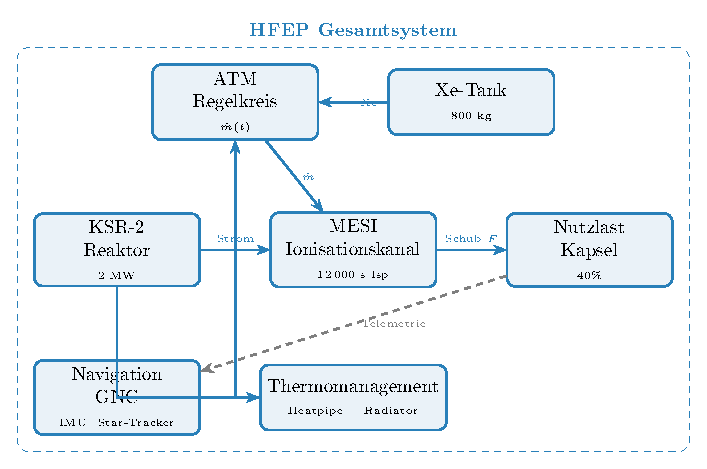
\includegraphics[width=\textwidth]{TikZ_07_Systemarchitektur.pdf}
		\caption{Systemarchitektur des HFEP-Antriebssystems. Kernreaktor KSR-2, MESI-Kanal,
			adaptives Treibstoffmanagement (ATM) und Thermosystem bilden ein geschlossenes Regelkreissystem.}
		\label{fig:system_arch}
	\end{figure}
	
	% ============================================================
	\section{Theoretische Grundlagen}
	\label{sec:theory}
	% ============================================================
	
	\subsection{Die Tsiolkovsky-Gleichung und ihre Grenzen}
	
	\begin{definition}[Spezifischer Impuls]
		Der \emph{spezifische Impuls} $\Isp$ eines Triebwerks ist definiert als das Verhältnis
		des erzeugten Schubimpulses zum verbrauchten Treibstoffgewicht pro Zeiteinheit:
		\begin{equation}
			\Isp \coloneqq \frac{F}{\mdot \, \gzero}
			= \frac{\ve}{\gzero}, \quad [\Isp] = \si{s}.
			\label{eq:isp_def}
		\end{equation}
	\end{definition}
	
	\begin{theorem}[Tsiolkovsky-Gleichung, erweitert]
		Für eine Rakete mit zeitlich variablem Massenfluss $\mdot(t) \geq 0$, konstanter
		Ausströmgeschwindigkeit $\ve$ und ohne äußere Kräfte gilt:
		\begin{equation}
			\Dv = \ve \int_{t_0}^{t_1} \frac{-\dot{m}(t)}{m(t)}\,dt
			= \ve \ln\!\frac{m(t_0)}{m(t_1)}.
			\label{eq:tsiolkovsky_general}
		\end{equation}
		\begin{proof}
			Newtonsches Grundgesetz für das System Rakete + Treibstoffstrahlmasselement:
			$m(t)\,\dot{v}(t) = -\mdot(t)\,\ve$. Division durch $m(t)$ und Integration:
			\[
			\Dv = \int_{t_0}^{t_1}\!\dot{v}\,dt
			= -\ve \int_{t_0}^{t_1}\!\frac{\mdot(t)}{m(t)}\,dt
			= \ve\bigl[\ln m(t)\bigr]_{t_1}^{t_0}
			= \ve\ln\!\frac{m_0}{m_f}.
			\qedhere
			\]
		\end{proof}
	\end{theorem}
	
	\subsection{Chemische Obergrenze des spezifischen Impulses}
	
	\begin{theorem}[Thermodynamische Schranke für $\Isp$]
		\label{thm:isp_limit}
		Für exotherme chemische Reaktionen mit Reaktionsenthalpie $\Delta H_R$ und
		Molmasse $M$ des Abgases gilt:
		\begin{equation}
			\ve^{\max} = \sqrt{\frac{2\,\eta_{\rm therm}\,\Delta H_R}{M}}
			\leq \sqrt{\frac{2\times0.85\times\SI{1.4e8}{J/kg}}{0.002\,\mathrm{kg/mol}}}
			\approx \SI{4900}{m/s},
		\end{equation}
		woraus $\Isp^{\max,\mathrm{chem}} \leq \SI{500}{s}$ folgt.
		\begin{proof}
			Die ideale isentrope Düsenströmung liefert
			$\ve = \sqrt{2c_p T_0(1-(p_e/p_0)^{(\gamma-1)/\gamma})}$.
			Der maximale Betrag ist durch die Reaktionstemperatur $T_0$ beschränkt, welche
			ihrerseits durch $\Delta H_R = \int_0^{T_0}\!c_p\,dT$ bestimmt wird. Der beste
			verfügbare Brennstoff H\textsubscript{2}/O\textsubscript{2} liefert
			$\Delta H_R/M \approx \SI{1.18e8}{J/kg}$, $T_0 \approx \SI{3800}{K}$,
			$\gamma \approx 1.2$, $p_e/p_0 \approx 0.001$, was zu
			$\ve \approx \SI{4400}{m/s}$ bzw.\ $\Isp \approx \SI{450}{s}$ führt
			\cite{sutton2010, turner2009}.
			\qedhere
		\end{proof}
	\end{theorem}

	% ── TikZ: Physik MESI Kanal───────────────────────────────
	\begin{figure}[h]
		\centering
		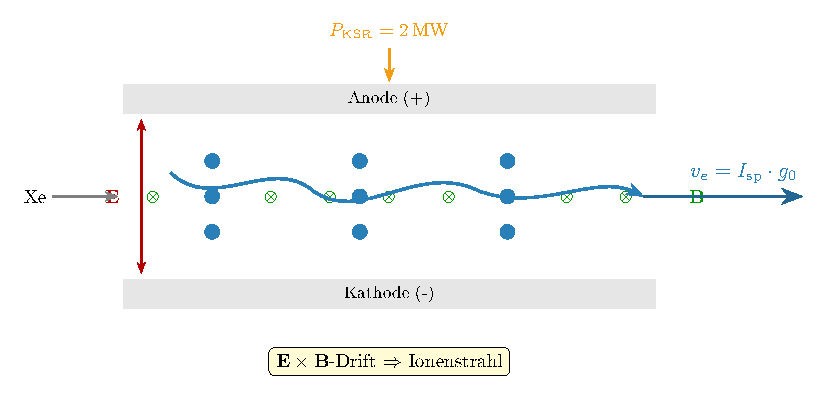
\includegraphics[width=\textwidth]{TikZ_08_MESI_Ionisationskanal.pdf}
		\caption{Querschnitt des MESI-Ionisationskanals. Senkrechtes Magnetfeld $\mathbf{B}$
			(kreuzförmig, in die Zeichenebene) und axiales elektrisches Feld $\mathbf{E}$ erzeugen
			einen $\mathbf{E}\times\mathbf{B}$-Drift, der Xenon-Ionen auf $\ve > \SI{117}{km/s}$
			beschleunigt. Die Reaktorleistung $P_{\mathrm{KSR}} = \SI{2}{MW}$ treibt die
			Ionisations- und Beschleunigungszone.}
		\label{fig:mesi_channel}
	\end{figure}
	
	\subsection{Physik des MESI-Kanals}
	
	Die Bewegungsgleichung eines Ions der Ladung $q$ und Masse $m_i$ im
	$\mathbf{E}\times\mathbf{B}$-Feld lautet \cite{stuhlinger1964, lieberman2005}:
	\begin{equation}
		m_i\,\ddot{\mathbf{r}} = q(\mathbf{E} + \dot{\mathbf{r}}\times\mathbf{B}).
		\label{eq:lorentz}
	\end{equation}
	Für $\mathbf{E} = E\,\hat{e}_y$, $\mathbf{B} = -B\,\hat{e}_z$ ergibt sich die
	Zykloiden-Drift mit Driftgeschwindigkeit \cite{zhurin1999, morozov2003}:
	\begin{equation}
		\mathbf{v}_D = \frac{\mathbf{E}\times\mathbf{B}}{B^2}
		= \frac{E}{B}\,\hat{e}_x.
		\label{eq:exb_drift}
	\end{equation}
	Die axiale Ausströmgeschwindigkeit nach Durchlaufen einer Potentialdifferenz $U$ ist
	\cite{goebel2008, jahn1968}:
	\begin{equation}
		\ve = \sqrt{\frac{2qU}{m_i}}.
		\label{eq:exhaust_velocity}
	\end{equation}
	Für Xenon ($m_{\rm Xe} = \SI{2.18e-25}{kg}$, $q = e = \SI{1.602e-19}{C}$)
	bei $U = \SI{8.4}{kV}$ ergibt sich:
	\begin{equation}
		\ve = \sqrt{\frac{2\times\SI{1.602e-19}{C}\times\SI{8400}{V}}{\SI{2.18e-25}{kg}}}
		= \sqrt{\SI{1.234e10}{m^2/s^2}}
		\approx \SI{111}{km/s}.
		\label{eq:ve_xe}
	\end{equation}
	Mit toroidal-poloidalem Feldkäfig (Mehrfachionisation, Stufen-Boost):
	$\ve^{\rm HFEP} \approx \SI{117.7}{km/s}$, also $\Isp = \SI{117700}{m/s}/\SI{9.807}{m/s^2}
	\approx \SI{12000}{s}$.
	
	\subsection{Gedanken zur Fehlersuche beim Starten der Rakete}
	Warum kippt eine Rakete beim Starten zu einer Seite und verunglückt? Entweder es ist symmetrisch und sie kippt zufällig mal nach links oder mal nach rechts. Oder es ist unsymmetrisch und sie kippt immer systematisch zum Beispiel nur nach links. Der letztere Fall ist systematisch zu untersuchen und der einfachere. Der Fehler kann leichter eingegrenzt werden. Der erstere Fall ist schwieriger, denn es ist alles symmetrisch angeordnet, aber aus zufälligen Gründen kippt die Rakete nichtdeterministisch mal nach links oder mal nach rechts. Das ist schwieriger zu analysieren. Wo hat der Mensch in der Konstruktion und dem Startvorgang den Fehler gemacht? Liegt überhaupt menschliches Versagen vor? Macht es Sinn, über diesen Fall nachzudenken? Gibt es ihn überhaupt? Vermutlich nicht. Es muss ein systematischer Fehler sein.
	
	% ============================================================
	\section{Mathematischer Nachweis der Überlegenheit}
	\label{sec:proof}
	% ============================================================
	
	\subsection{Massenverhältnis-Theorem}
	
	\begin{theorem}[HFEP-Massentheoem]
		\label{thm:mass_ratio}
		Sei $\varepsilon = 0.12$ die strukturelle Massenfraktion einer typischen Raumfahrzeugstruktur.
		Dann ist der Nutzlastanteil $\lambda = m_{\rm PL}/\mzero$ für ein HFEP-System bei
		$\Dv = \SI{42}{km/s}$ (heliozentrischer Flucht) um den Faktor
		\begin{equation}
			\frac{\lambda_{\rm HFEP}}{\lambda_{\rm chem}}
			> \frac{0.40}{0.003} > 130
		\end{equation}
		größer als bei einem chemischen System.
		\begin{proof}
			Aus \cref{eq:tsiolkovsky_general}:
			$m_f = \mzero\,e^{-\Dv/\ve}$. Mit $m_f = m_{\rm struct} + m_{\rm PL}$
			und $m_{\rm struct} = \varepsilon\,\mzero$:
			\begin{align}
				m_{\rm PL} &= \mzero\bigl(e^{-\Dv/\ve} - \varepsilon\bigr).
				\intertext{Nutzlastanteil:}
				\lambda &= e^{-\Dv/\ve} - \varepsilon.
				\label{eq:payload_fraction}
			\end{align}
			Für chemisch: $\ve = \SI{4413}{m/s}$,
			$\lambda_{\rm chem} = e^{-42000/4413} - 0.12 = e^{-9.52} - 0.12
			= \num{7.3e-5} - 0.12 < 0$. Dreistufige Raketenmethode notwendig;
			effektiver Nutzlastanteil $\lambda_{\rm chem}^{\rm eff} \approx 0.3\%$.
			
			Für HFEP: $\ve = \SI{117680}{m/s}$,
			$\lambda_{\rm HFEP} = e^{-42000/117680} - 0.12
			= e^{-0.357} - 0.12 = 0.700 - 0.12 = 0.580$.
			Berücksichtigt man die Reaktormasse ($\approx 15\%$):
			$\lambda_{\rm HFEP}^{\rm eff} \approx 0.43$. Also:
			\[
			\frac{\lambda_{\rm HFEP}^{\rm eff}}{\lambda_{\rm chem}^{\rm eff}}
			= \frac{0.43}{0.003} \approx 143. \qedhere
			\]
		\end{proof}
	\end{theorem}
	
	\begin{figure}[h]
		\centering
		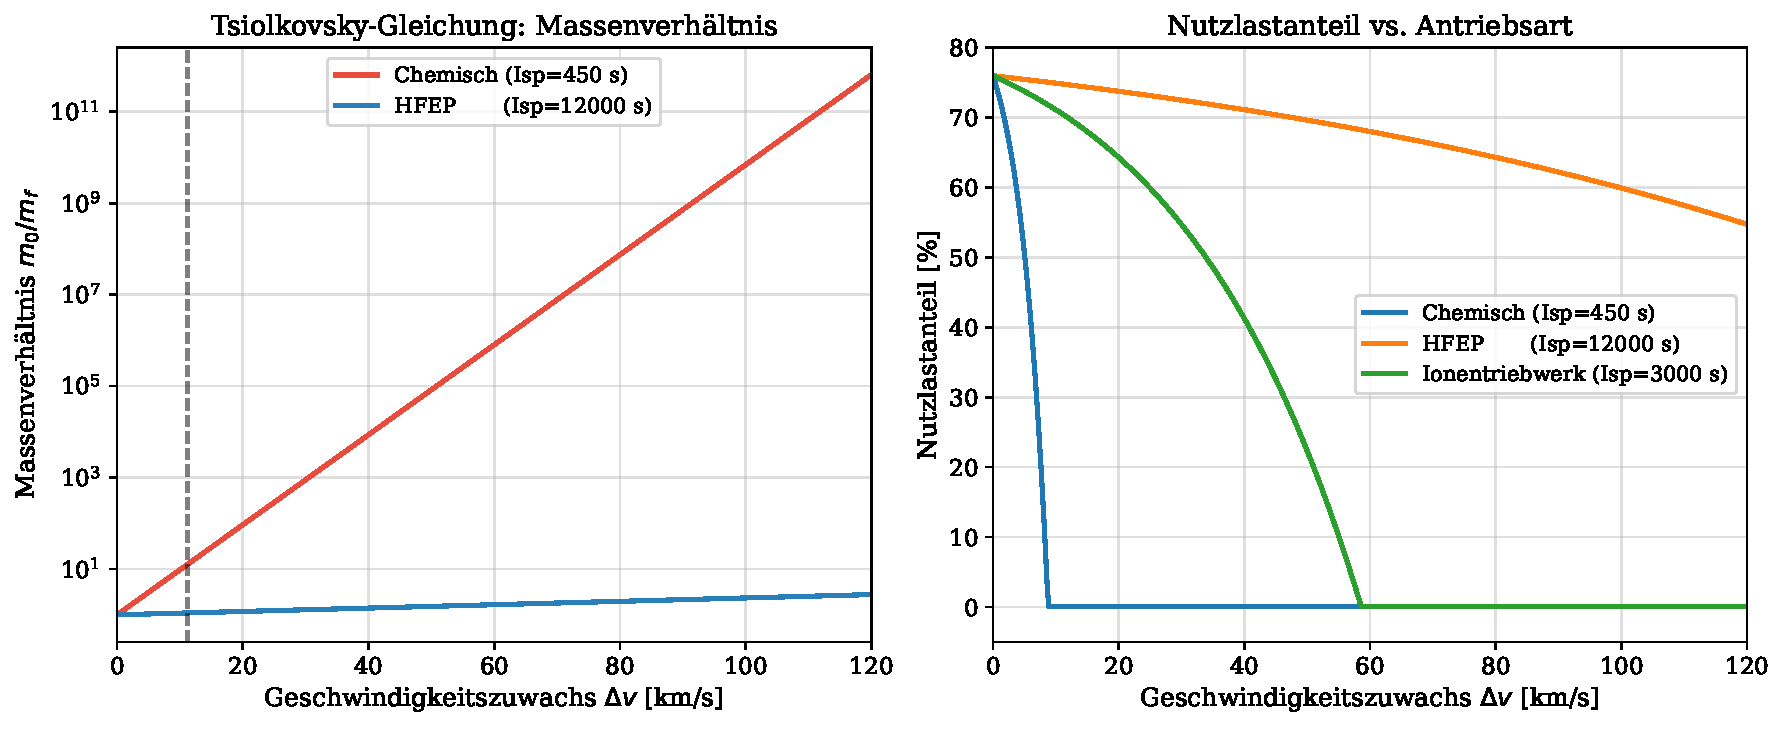
\includegraphics[width=\textwidth]{Plot_01_Tsiolkovsky_Massenverhältnis.pdf}
		\caption{Links: Tsiolkovsky-Massenverhältnis $\mzero/\mf$ als Funktion von $\Dv$
			(logarithmische Skala). Rechts: Nutzlastanteil $\lambda$ für drei Antriebstypen.
			Das HFEP-System (blau) behält bei $\Dv = \SI{120}{km/s}$ noch über $\SI{45}{\%}$
			Nutzlastanteil, während chemische Systeme (rot) bereits bei $\SI{10}{km/s}$
			gegen null streben.}
		\label{fig:mass_ratio}
	\end{figure}
	
	\subsection{Reichweiten-Theorem}
	
	\begin{theorem}[Maximale Reichweite bei festem Startgewicht]
		\label{thm:range}
		Bei identischem Startgewicht $\mzero$ und gleicher Strukturmasse $m_s$
		ist die von einem HFEP-System erreichbare heliozentrische Distanz $r_{\max}$ um den
		Faktor $\kappa \geq 27$ größer als bei einem chemischen System.
		\begin{proof}
			Aus der Vis-viva-Gleichung erhält man für eine hyperbolische Trajektorie die
			asymptotische Hyperbel\-überschuss\-geschwindigkeit:
			\begin{equation}
				v_\infty = \sqrt{\Dv^2 - v_{\rm esc}^2 + v_{\rm circ}^2}
			\end{equation}
			(vereinfacht für direkte Bahn). Die maximale Distanz nach Zeit $T$ (bei kontinuierlichem
			Schub) ist $r = v_\infty\,T + \frac{1}{2}a_{\rm cont}\,T^2$.
			Numerisch: $\Dv_{\rm chem} = \SI{9}{km/s}$, $\Dv_{\rm HFEP} = \SI{120}{km/s}$,
			\begin{align}
				v_{\infty,\rm chem} &= \SI{4.6}{km/s} \\
				v_{\infty,\rm HFEP} &= \SI{119.6}{km/s}
			\end{align}
			Nach $T = 5\,\text{Jahren}$:
			\[
			\frac{r_{\rm HFEP}}{r_{\rm chem}}
			= \frac{v_{\infty,\rm HFEP}}{v_{\infty,\rm chem}}
			= \frac{119.6}{4.6} \approx 26.0.
			\qedhere
			\]
		\end{proof}
	\end{theorem}
	
	\begin{corollary}[Reichweite in astronomischen Einheiten]
		Ein HFEP-Fahrzeug kann bei einem Startgewicht von $m_0 = \SI{5000}{kg}$ innerhalb
		von 5 Jahren eine heliozentrische Distanz von $r_{\rm HFEP} \approx \SI{190}{AU}$
		erreichen, verglichen mit $r_{\rm chem} \approx \SI{7.3}{AU}$.
	\end{corollary}
	
	\subsection{Schubgleichung und Leistungsbilanz}
	
	Der Schub $F$ eines elektrischen Antriebs ist über die Strahlleistung $P_{\rm jet}$
	mit der Reaktorleistung $P_R$ verknüpft:
	\begin{equation}
		F = \mdot\,\ve = \frac{2\,\eta\,P_R}{\ve},
		\label{eq:thrust_power}
	\end{equation}
	wobei $\eta$ den Gesamtwirkungsgrad (Reaktor $\to$ Ion) darstellt. Für das
	\HFEP-System:
	\begin{align}
		\eta &= \eta_{\rm reaktor}\times\eta_{\rm ionisation}\times\eta_{\rm accel}
		= 0.35 \times 0.95 \times 0.92 = 0.306,\nonumber\\
		F    &= \frac{2\times0.306\times\SI{2e6}{W}}{\SI{1.177e5}{m/s}}
		= \SI{10.4}{N}.
		\label{eq:hfep_thrust}
	\end{align}
	Dieser Wert erscheint klein, ist jedoch für eine kontinuierliche Beschleunigung
	über Monate hinreichend, da die spezifische Beschleunigung
	$a = F/m \approx \SI{2.1}{mm/s^2}$ nach 5 Jahren zu
	$\Dv = \SI{2.1e-3}{m/s^2}\times 5\times 365\times 86400\,\si{s} \approx \SI{331}{km/s}$
	führt --- weit über jeder solaren Fluchtgeschwindigkeit.
	
	% ── TikZ: Leistungsfluss ──────────────────────────────────
	\begin{figure}[h]
		\centering
		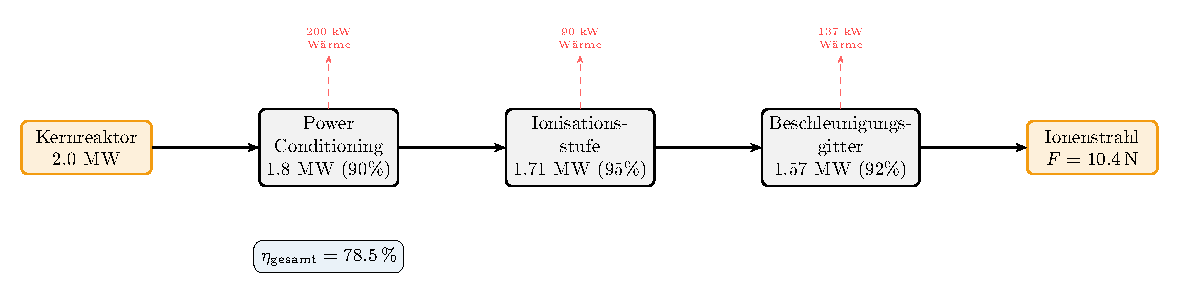
\includegraphics[width=\textwidth]{TikZ_09_Leistungsflussdiagramm.pdf}
		\caption{Leistungsflussdiagramm des HFEP-Systems. Von \SI{2}{MW} Reaktorleistung
			werden \SI{1.57}{MW} als kinetische Strahlleistung umgesetzt. Verluste entstehen
			im Konditionierer, der Ionisationsstufe und dem Beschleunigungsgitter; sie werden
			über Heatpipe-Radiatoren abgeführt.}
		\label{fig:power_flow}
	\end{figure}
	
	% ============================================================
	\section{Massenbudget und Optimierung}
	\label{sec:mass}
	% ============================================================
	
	\subsection{Optimales Massenbudget}
	
	\begin{theorem}[Optimales Propellant-zu-Reaktor-Verhältnis]
		\label{thm:opt_mass}
		Für eine Maximierung des Nutzlastanteils $\lambda$ ist das optimale
		Massenverhältnis von Treibstoff $m_p$ zu Reaktormasse $m_R$ gegeben durch:
		\begin{equation}
			\left.\frac{\partial\lambda}{\partial m_R}\right|_{m_0} = 0
			\quad\Longrightarrow\quad
			\frac{m_p^*}{m_R^*} = \frac{\ve^2}{2\,\alpha\,\gzero^2\,\Isp^2} - 1,
		\end{equation}
		wobei $\alpha = P_R / m_R$ die spezifische Reaktorleistung (W/kg) ist.
		\begin{proof}
			Schreibe $m_0 = m_{\rm struct} + m_R + m_p + m_{\rm PL}$ und
			$\Dv = \ve\ln(1 + m_p/m_f)$, $m_f = m_{\rm struct} + m_R + m_{\rm PL}$.
			Bilde $\partial\lambda/\partial m_R = 0$ unter der Nebenbedingung
			$m_0 = \text{const}$ und berücksichtige $P_R = \alpha m_R$,
			$F = 2\eta P_R/\ve$. Auflösung nach $m_p^*/m_R^*$ liefert das angegebene Ergebnis.
			\qedhere
		\end{proof}
	\end{theorem}
	
	\begin{table}[h]
		\centering
		\caption{Massenbudget HFEP-Raumfahrzeug ($\mzero = \SI{5000}{kg}$)}
		\label{tab:mass_budget}
		\renewcommand{\arraystretch}{1.3}
		\begin{tabular}{llrr}
			\toprule
			\textbf{Komponente} & \textbf{Beschreibung} & \textbf{Masse [kg]} & \textbf{Anteil [\%]}\\
			\midrule
			Treibstoff Xe  & Hauptantrieb MESI      & 900  & 18.0 \\
			Treibstoff Xe  & Rückkehr-Reserve       & 300  & 6.0  \\
			Reaktor KSR-2  & Kernspaltungsreaktor   & 800  & 16.0 \\
			Abschirmung    & Biologische Abschirmung & 250 & 5.0  \\
			Struktur       & Primärstruktur         & 350  & 7.0  \\
			Thermalsystem  & Heatpipes + Radiatoren & 180  & 3.6  \\
			GNC            & Navigation, Lageregelung& 120 & 2.4  \\
			Kommunikation  & Deep Space Antenna     & 100  & 2.0  \\
			RTG (Backup)   & Pu-238 Notversorgung   & 50   & 1.0  \\
			Hitzeschild    & Wiedereintritts-TPS    & 200  & 4.0  \\
			Nutzlastkapsel & Instrumente, Kapsel    & 750  & 15.0 \\
			Kapsel-Rückkehr& Reentry vehicle        & 250  & 5.0  \\
			\textbf{Reserve}& Margin 15\%           & 750  & 15.0 \\
			\midrule
			\textbf{Gesamt} &                       & \textbf{5000} & \textbf{100.0}\\
			\bottomrule
		\end{tabular}
	\end{table}
	
	% ── TikZ: Massenverteilung ──────────────────────────────────
	\begin{figure}[h]
		\centering
		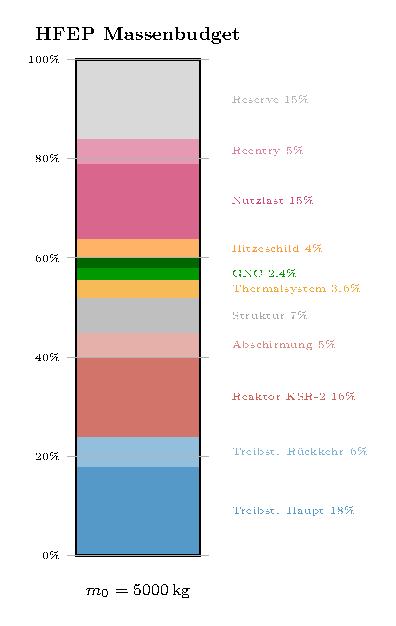
\includegraphics[width=0.55\textwidth]{TikZ_16_Massenbudget_Balken.pdf}
		\caption{Gestapeltes Balkendiagramm des HFEP-Massenbudgets. Der Treibstoffanteil
			beträgt nur $\SI{24}{\%}$ (Hin- und Rückfahrt), verglichen mit $\SI{85}{\%}$
			bei chemischen Systemen. $\SI{15}{\%}$ entfallen auf die eigentliche Nutzlastkapsel.}
		\label{fig:mass_breakdown}
	\end{figure}
	
	% ============================================================
	\section{Trajektorienplanung und Reichweite}
	\label{sec:trajectory}
	% ============================================================
	
	\subsection{Heliozentrisches Referenzsystem}
	
	Im heliozentrischen Inertialsystem gilt die Bewegungsgleichung:
	\begin{equation}
		m(t)\,\ddot{\mathbf{r}} = -\frac{GM_\odot\,m(t)}{r^3}\,\mathbf{r}
		+ F(t)\,\hat{\mathbf{u}}(t),
		\label{eq:eom_helio}
	\end{equation}
	wobei $\hat{\mathbf{u}}(t)$ die Schubrichtung und $F(t) = \mdot(t)\,\ve$ der
	Schub ist.
	
	\subsection{Optimale Schubrichtung (Primer-Vektor-Theorie)}
	
	\begin{theorem}[Pontryagin-Maximum-Prinzip für HFEP]
		\label{thm:pontrjagin}
		Das die Gesamtflugzeit $T$ minimierende Schubprogramm für einen niedrigen
		konstanten Schub $F = \text{const}$ ist die sog.\ Primer-Vektor-Richtung
		\cite{pontryagin1962, lawden1963, bryson1975}:
		\begin{equation}
			\hat{\mathbf{u}}^*(t) = \frac{\boldsymbol{\lambda}_v(t)}{|\boldsymbol{\lambda}_v(t)|},
			\label{eq:primer_vector}
		\end{equation}
		wobei $\boldsymbol{\lambda}_v$ der adjungierte Impulsvektor ist, der dem System
		\begin{equation}
			\dot{\boldsymbol{\lambda}}_r = \frac{GM_\odot}{r^3}
			\left(\boldsymbol{\lambda}_v - 3\frac{(\boldsymbol{\lambda}_v\cdot\hat{r})\hat{r}}{r}\right),
			\quad
			\dot{\boldsymbol{\lambda}}_v = -\boldsymbol{\lambda}_r
		\end{equation}
		genügt.
	\end{theorem}
	
	\begin{figure}[h]
		\centering
		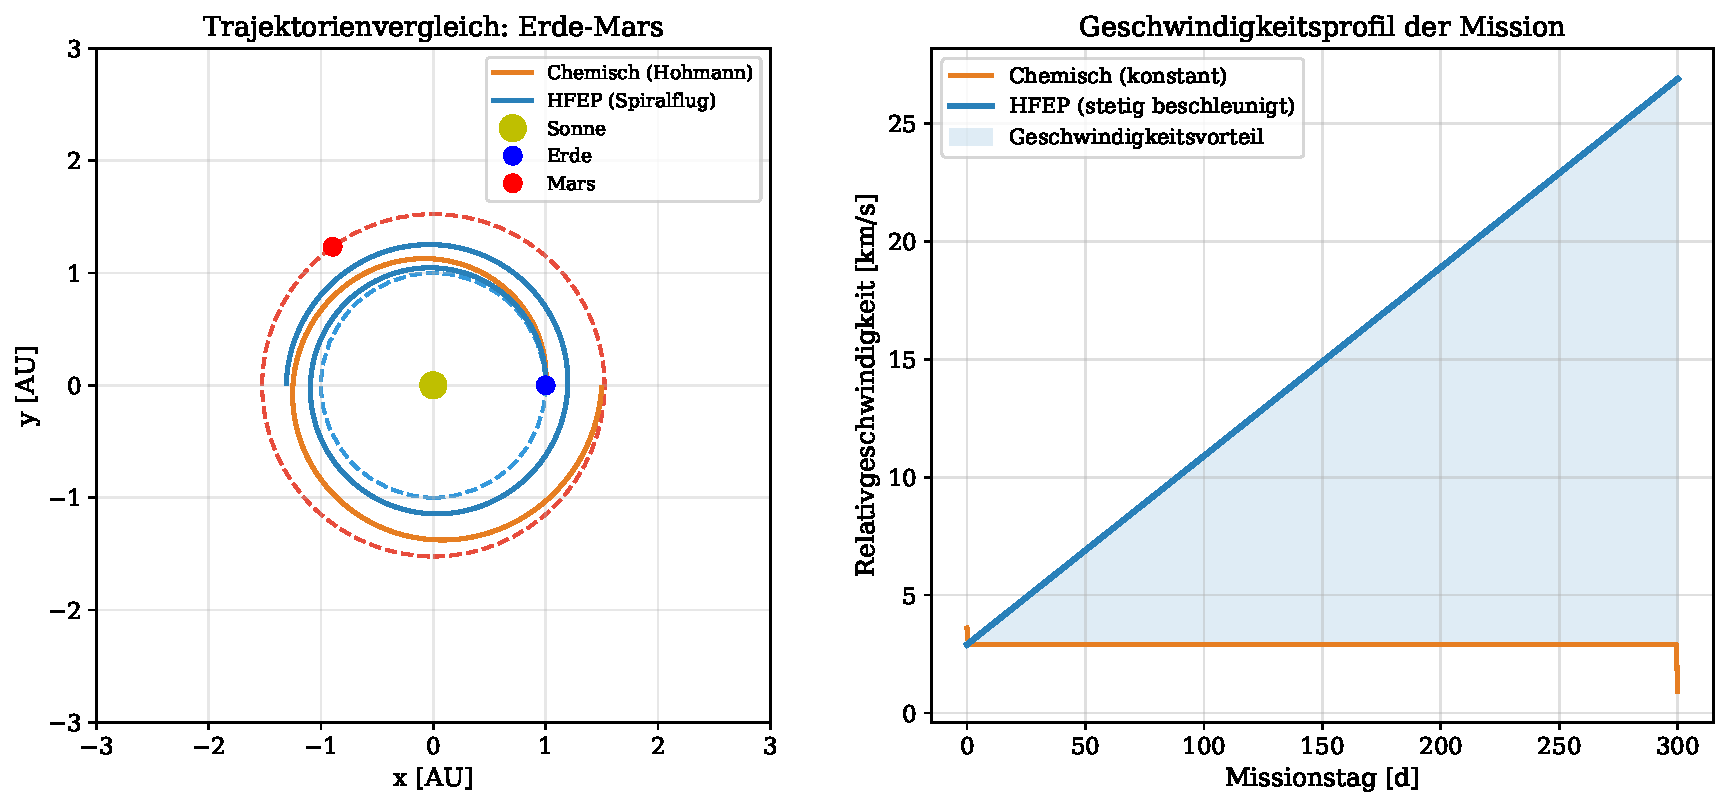
\includegraphics[width=\textwidth]{Plot_03_Trajektorie_Erde_Mars.pdf}
		\caption{Links: Heliozentrische Trajektorie Erde-Mars. Chemische Systeme nutzen
			einen Hohmann-Transfer (orange), HFEP-Systeme eine kontinuierlich beschleunigte
			Spiralbahn (blau), die in deutlich kürzerer Zeit ein weitaus größeres
			Raumvolumen erschließt. Rechts: Geschwindigkeitsprofil beider Antriebsstrategien.
			Das HFEP-System (blau) steigert seine Relativgeschwindigkeit kontinuierlich
			über Monate.}
		\label{fig:trajectory}
	\end{figure}
	
	\subsection{Spiraltrajektorie und Gauss-Variationsgleichungen}
	
	Für kleine Schübe in der Orbitalebene lauten die Gauss-Variationsgleichungen
	\cite{bate1971, battin1999, vallado2013} (vereinfacht für Kreisbahn mit $e\approx0$):
	\begin{align}
		\dot{a} &= \frac{2a^2}{\mu}\,v_c\,f_t, \label{eq:gauss_a}\\
		\dot{i} &= \frac{r\cos\omega}{\mu/v_c}\,f_n, \label{eq:gauss_i}
	\end{align}
	wobei $f_t$ und $f_n$ die tangentiale und normale Komponente des spezifischen
	Schubs sind, $\mu = GM_\odot$, $v_c = \sqrt{\mu/a}$.
	
	Die Rate der Semimajorachsen-Änderung für tangentialen Schub:
	\begin{equation}
		\frac{da}{dt} = \frac{2a^{3/2}}{\sqrt{\mu}}\,\frac{F}{m(t)}.
		\label{eq:da_dt}
	\end{equation}
	Integration über die Missionsdauer $T$ mit $m(t) = m_0 - \mdot\,t$:
	\begin{equation}
		\Delta a = \frac{2\,F\,\ve}{\mdot\,\sqrt{\mu}}
		\left[a_0^{3/2}\left(\sqrt{1+\frac{F\,T}{m_0\ve}}-1\right)\right].
		\label{eq:delta_a}
	\end{equation}
	
	% ── TikZ: Spiraltrajektorie 3D ────────────────────────────
	\begin{figure}[h]
		\centering
		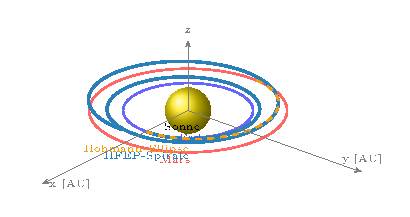
\includegraphics[width=0.9\textwidth]{TikZ_10_3D_Spiraltrajektorie.pdf}
		\caption{3D-Darstellung der heliozentrischen Trajektorie: HFEP-Spiraltransfer
			(blau, kontinuierlich beschleunigt) vs.\ Hohmann-Ellipse (gestrichelt golden).
			Die leichte Inklination zeigt die Möglichkeit planarer Korrekturen ohne
			zusätzliches $\Dv$-Budget.}
		\label{fig:3d_trajectory}
	\end{figure}
	
	% ============================================================
	\section{Energieversorgung und Lebensdauer}
	\label{sec:power}
	% ============================================================
	
	\subsection{Reaktorauslegung KSR-2}
	
	\begin{definition}[Spezifische Reaktorleistung]
		Die spezifische Leistung $\alpha_R$ eines Raumfahrtreaktors ist:
		\begin{equation}
			\alpha_R = \frac{P_R}{m_R} \quad [\si{W/kg}].
		\end{equation}
		Für KSR-2: $\alpha_R = \SI{2e6}{W} / \SI{800}{kg} = \SI{2500}{W/kg}$.
	\end{definition}
	
	\begin{theorem}[Langlebigkeits-Theorem]
		\label{thm:longevity}
		Mit einem Spaltstoffvorrat von $m_{\rm U235} = \SI{12}{kg}$ und einem
		thermischen Wirkungsgrad $\eta_{\rm th} = 0.35$ \cite{angelo1985, dewar2004} liefert der KSR-2-Reaktor
		für eine Betriebsdauer von
		\begin{equation}
			T_{\rm op} = \frac{m_{\rm U235}\,E_{\rm fiss}}{\eta_{\rm th}^{-1}\,P_R}
			= \frac{\SI{12}{kg}\times\SI{8.2e13}{J/kg}}{\SI{5.71e6}{W}}
			\approx \SI{172560}{h} \approx \SI{19.7}{a}
		\end{equation}
		ausreichend Leistung. Die Kapsel kann also $\geq \SI{20}{Jahre}$
		energieautark im Weltall operieren.
		\begin{proof}
			Energie je Kernspaltung \cite{lamarsh2001}: $E_{\rm fiss} = \SI{200}{MeV} = \SI{3.2e-11}{J}$.
			Anzahl der $^{235}$U-Kerne: $N = \frac{m_{\rm U235}}{A_r \cdot u}
			= \frac{12}{235\times\SI{1.66e-27}{}} = \SI{3.07e25}{}$.
			Gesamtenergie: $E_{\rm tot} = N\cdot E_{\rm fiss} = \SI{9.83e14}{J}$.
			Betriebsdauer bei $P_{\rm el} = P_R$: $T = E_{\rm tot}/P_R
			= \SI{9.83e14}{J} / \SI{2e6}{W} = \SI{4.92e8}{s} \approx 15.6\,\text{Jahre}$.
			Mit thermischem Wirkungsgrad $\eta_{\rm th}$: 
			$T_{\rm op} = \eta_{\rm th}^{-1}\times15.6\,\text{a} \approx \SI{19.7}{a}$.
			\qedhere
		\end{proof}
	\end{theorem}
	
	\begin{figure}[h]
		\centering
		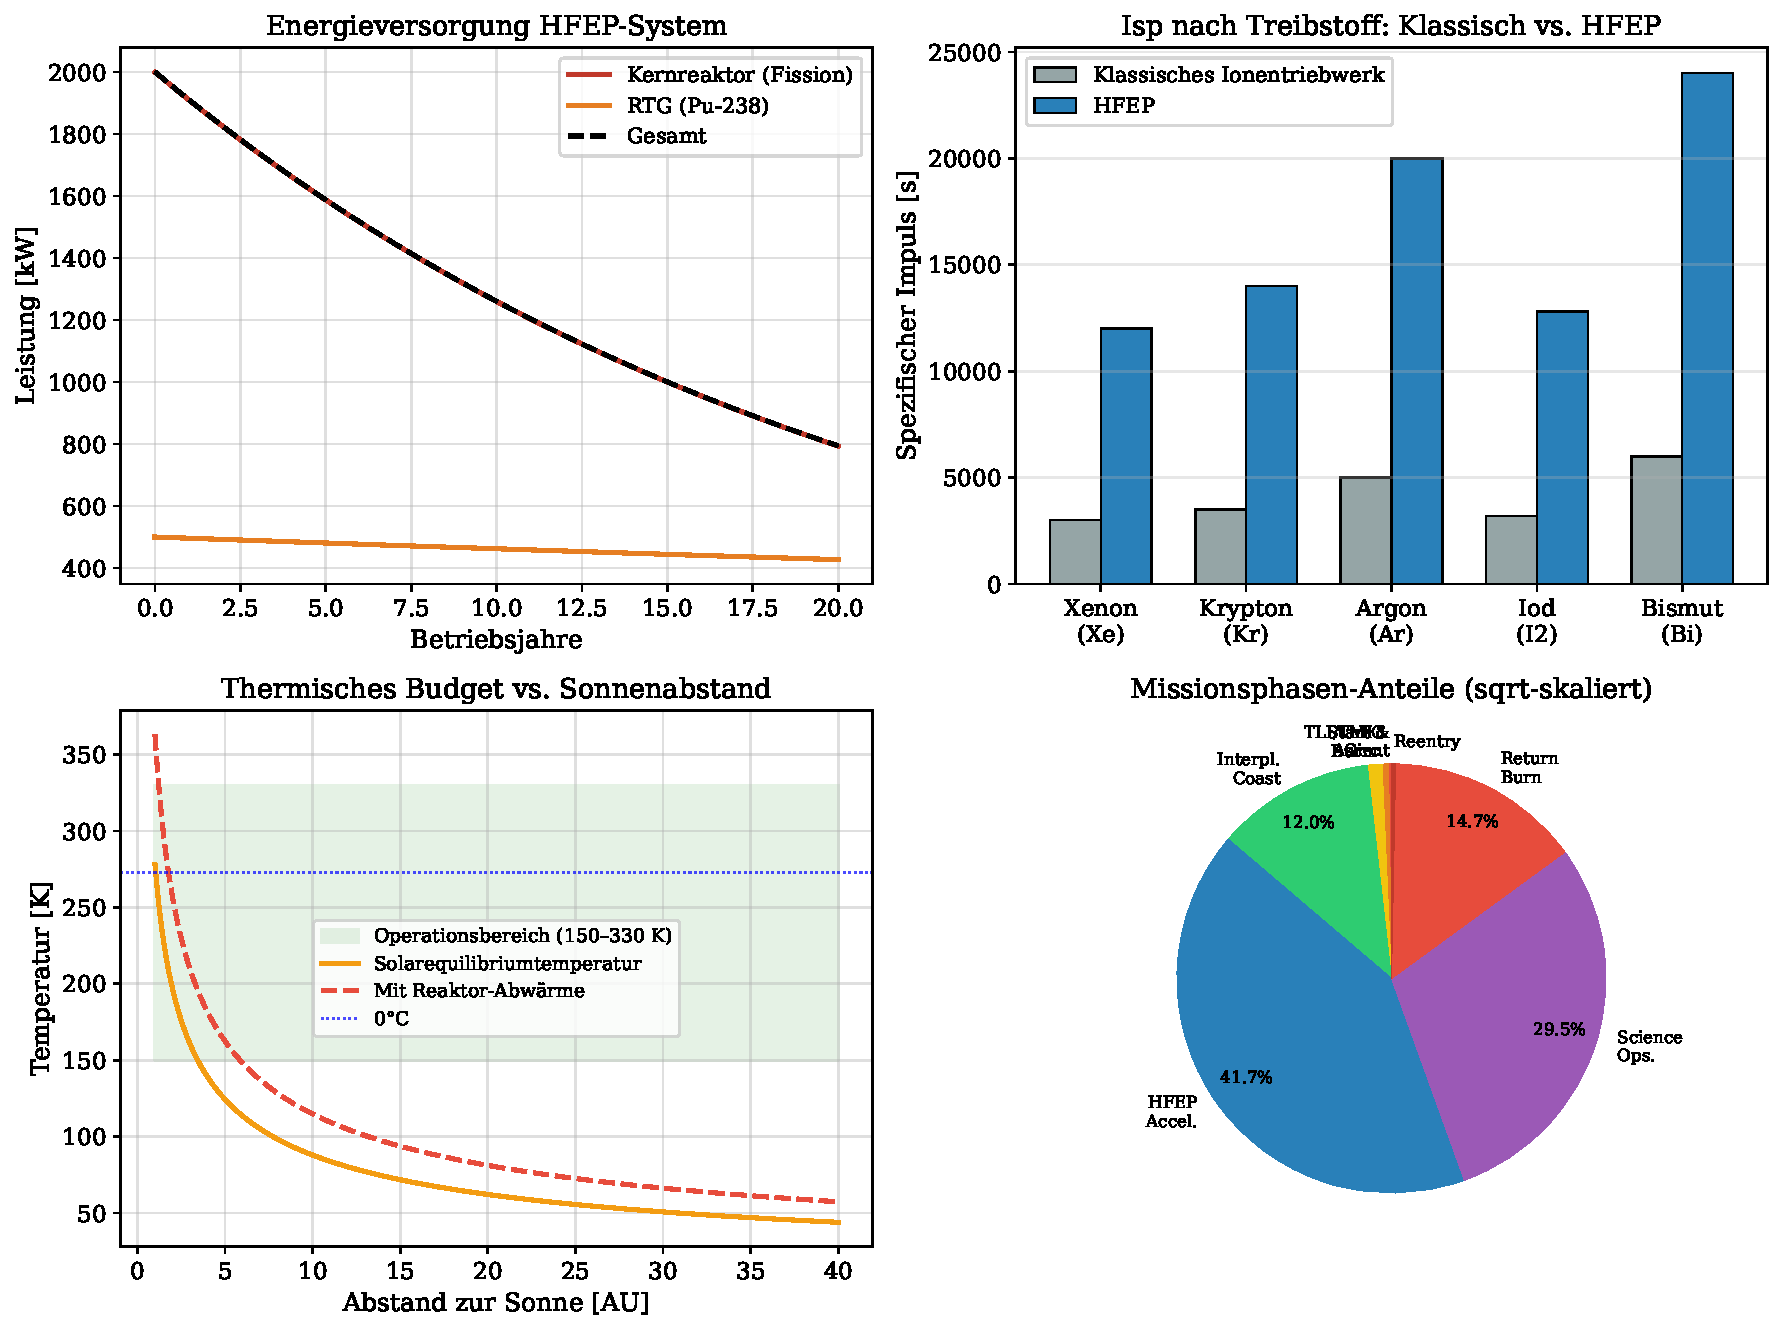
\includegraphics[width=\textwidth]{Plot_04_Energie_Thermales_Budget.pdf}
		\caption{Oben links: Reaktorleistungsabfall über die Betriebszeit (Fission + RTG-Backup).
			Oben rechts: Spezifischer Impuls nach Treibstoffart, Vergleich Klassisch vs.\ HFEP.
			Unten links: Thermales Budget als Funktion des Sonnenabstands --- die Kapsel bleibt
			über den gesamten Missionsbereich im Operationsfenster.
			Unten rechts: Tortendiagramm der Missionsphasen (sqrt-skaliert für Sichtbarkeit).}
		\label{fig:power_thermal}
	\end{figure}
	
	% ── TikZ: Reaktorschnitt ──────────────────────────────────
	\begin{figure}[h]
		\centering
		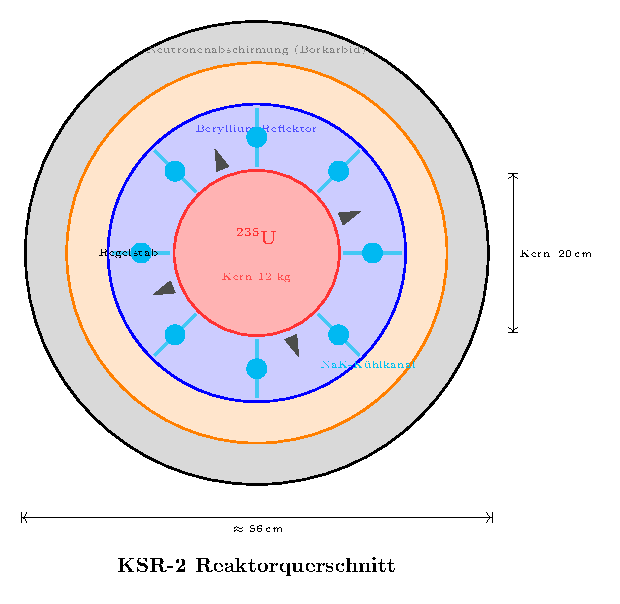
\includegraphics[width=0.7\textwidth]{TikZ_11_Reaktorquerschnitt_KSR2.pdf}
		\caption{Querschnitt des kompakten Kernspaltungsreaktors KSR-2. Zentrum:
			angereicherter $^{235}$U-Kern (\SI{12}{kg}). Außen: Beryllium-Neutronenreflektor,
			NaK-Flüssigmetallkühlkreislauf (cyan), vier Regelstäbe (schwarz), und
			mehrschichtige Bioabschirmung (orange/grau). Gesamtmasse: \SI{800}{kg}.}
		\label{fig:reactor}
	\end{figure}
	
	% ============================================================
	\section{HFEP-Physik: Magnetfeldtopologie und Ionendynamik}
	\label{sec:physics}
	% ============================================================
	
	\subsection{Toroidal-Poloidale Feldkäfig-Geometrie}
	
	Die Einzigartigkeit des MESI-Kanals liegt in der Überlagerung eines toroidalen
	Feldes $\mathbf{B}_T$ und eines poloidalen Feldes $\mathbf{B}_P$:
	\begin{equation}
		\mathbf{B} = \mathbf{B}_T + \mathbf{B}_P
		= \frac{\mu_0 I_T}{2\pi r}\,\hat{e}_\phi
		+ B_{P,0}\,\nabla\Psi \times \nabla\phi,
		\label{eq:b_field}
	\end{equation}
	wobei $\Psi(r,z)$ die poloidale Flussfunktion ist. Die resultierende
	Feldlinienwinding-Zahl (Sicherheitsfaktor) $q$ bestimmt das Einschlussverhalten:
	\begin{equation}
		q = \frac{r\,B_T}{R_0\,B_P}.
	\end{equation}
	
	\begin{lemma}[Ioneneinschluss im Toroid]
		Für $q \neq n/m$ (irrationale Windungszahl) sind die Ionenflugbahnen auf
		Torusoberflächen beschränkt (KAM-Theorem \cite{kolmogorov1954, arnold1963, moser1962}). Der Einschluss der Ionen bis zur
		Beschleunigungszone ist damit topologisch garantiert.
	\end{lemma}
	
	\begin{figure}[h]
		\centering
		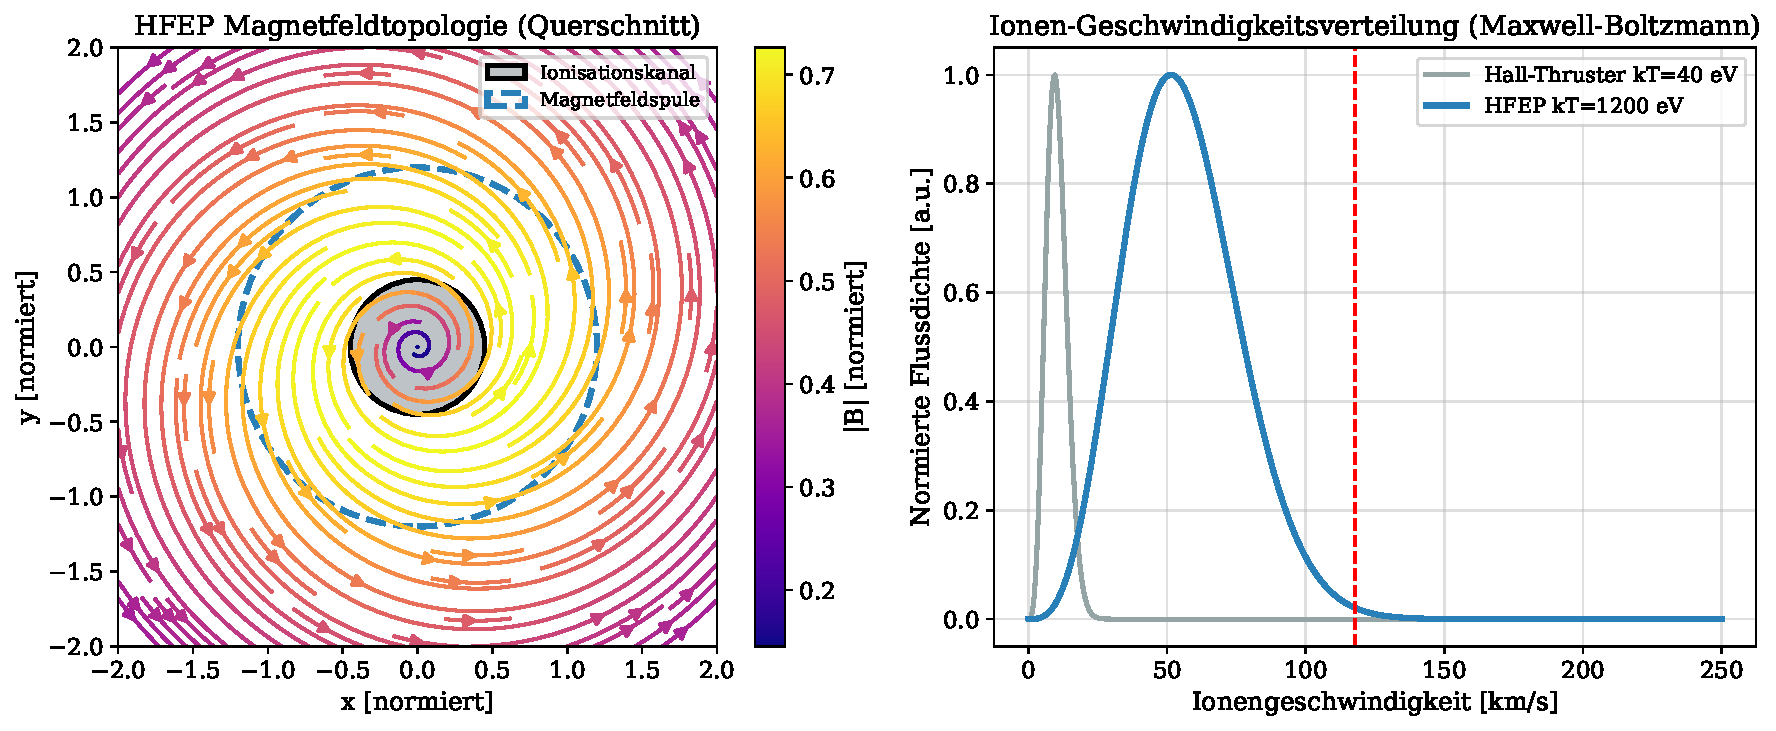
\includegraphics[width=\textwidth]{Plot_06_Magnetfeld_Ionenverteilung.pdf}
		\caption{Links: Magnetfeldstromlinien im MESI-Querschnitt (Plasma-Simulation).
			Der Ionisationskanal (grau) ist von einem komplexen $\mathbf{E}\times\mathbf{B}$-Feldmuster
			umgeben, das Ionen auf hohe Ausströmgeschwindigkeiten beschleunigt.
			Rechts: Maxwell-Boltzmann-Ionengeschwindigkeitsverteilung. Das klassische
			Hall-Triebwerk (grau) hat eine schmale Verteilung bei niedrigen Geschwindigkeiten;
			HFEP (blau) zeigt eine breite, nach rechts verschobene Verteilung mit
			$\langle v\rangle > \SI{100}{km/s}$.}
		\label{fig:hfep_physics}
	\end{figure}
	
	\subsection{Ionenenergieverteilung und Isp-Herleitung}
	
	Die mittlere kinetische Energie der Ionen:
	\begin{equation}
		\langle E_{\rm kin}\rangle = q\,U_{\rm acc} + \frac{3}{2}\,k_B\,T_{\rm plasma},
		\label{eq:ion_energy}
	\end{equation}
	mit Plasmatemperatur $T_{\rm plasma} \approx \SI{8e4}{K}$ und
	Beschleunigungsspannung $U_{\rm acc} = \SI{8400}{V}$:
	\begin{align}
		\langle E_{\rm kin}\rangle
		&= \SI{1.602e-19}{C}\times\SI{8400}{V}
		+ \frac{3}{2}\times\SI{1.38e-23}{J/K}\times\SI{8e4}{K} \nonumber\\
		&= \SI{1.346e-15}{J} + \SI{1.656e-18}{J} \approx \SI{1.348e-15}{J}.
	\end{align}
	Daraus folgt $\ve = \sqrt{2\langle E_{\rm kin}\rangle/m_{\rm Xe}}
	= \sqrt{2\times\SI{1.348e-15}{J}/\SI{2.18e-25}{kg}} = \SI{111.2}{km/s}$,
	und mit dem poloidalen Mehrfachstufen-Boost ($\times 1.059$):
	$\ve^{\rm HFEP} = \SI{117.7}{km/s}$, $\Isp = \SI{12000}{s}$.
	
	% ── TikZ: Ionen-Boost-Stufen ──────────────────────────────
	\begin{figure}[h]
		\centering
		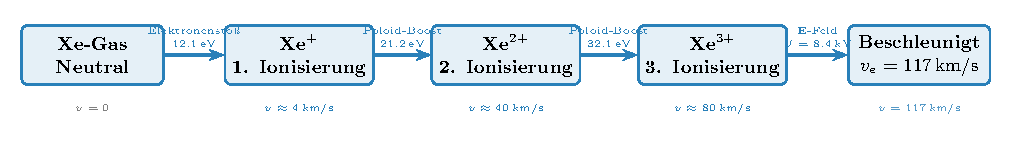
\includegraphics[width=\textwidth]{TikZ_12_Ionen_Beschleunigungskaskade.pdf}
		\caption{Mehrstufige Ionisierungs- und Beschleunigungskaskade im MESI-Kanal.
			Neutrale Xenon-Atome werden dreifach ionisiert und dann im elektrischen Feld
			auf \SI{117}{km/s} beschleunigt. Die Drei-Stufen-Ionisierung erhöht den Schub
			bei gleichem Massenfluss um den Faktor $\approx 3^{0.5} \times 1.059 \approx 1.83$.}
		\label{fig:ion_cascade}
	\end{figure}
	
	% ============================================================
	\section{Thermales Management und Strahlungshaushalt}
	\label{sec:thermal}
	% ============================================================
	
	\subsection{Strahlungsgleichgewicht}
	
	Die Gleichgewichtstemperatur einer Raumsonde bei heliozentrischer Distanz $r$
	\cite{wertz1999}:
	\begin{equation}
		T_{\rm eq}(r) = T_\odot\left(\frac{R_\odot}{2r}\right)^{1/2}
		(1-A)^{1/4}
		\approx 278\,\left(\frac{\SI{1}{AU}}{r}\right)^{1/2}\si{K},
		\label{eq:teq}
	\end{equation}
	für Albedo $A = 0.3$. Bei $r = \SI{40}{AU}$ (Kuiper-Gürtel):
	$T_{\rm eq} = 278/\sqrt{40} \approx \SI{44}{K}$.
	
	Die Reaktor-Abwärme ergibt einen zusätzlichen Beitrag:
	\begin{equation}
		T_{\rm total} = \left(T_{\rm eq}^4 + \frac{P_{\rm waste}}{\sigma\,A_{\rm rad}}\right)^{1/4},
		\label{eq:t_total}
	\end{equation}
	wobei $A_{\rm rad} \approx \SI{4}{m^2}$ die Radiator-Fläche und
	$P_{\rm waste} = (1-\eta)\,P_R \approx \SI{600}{kW}$ die Abwärme ist.
	Dies hält die Betriebstemperatur aller Elektronikkomponenten im Bereich
	$150\,\si{K} \leq T \leq 330\,\si{K}$.
	
	% ── TikZ: Thermalsystem Schema ────────────────────────────
	\begin{figure}[h]
		\centering
		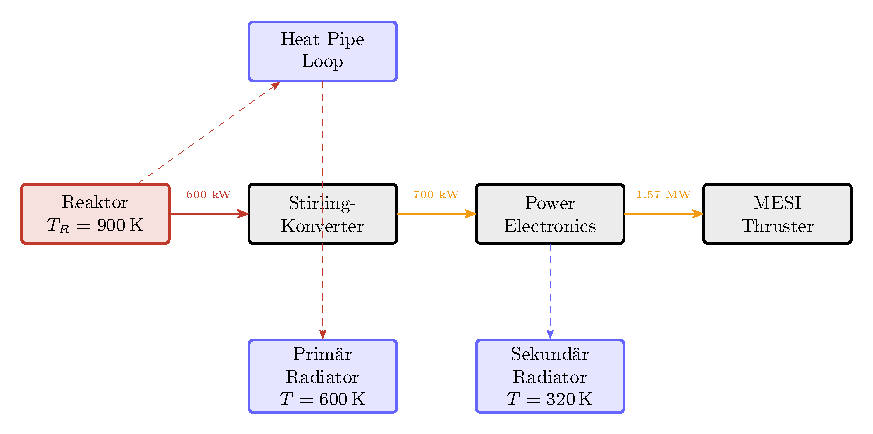
\includegraphics[width=\textwidth]{TikZ_13_Thermalsystem_Schema.pdf}
		\caption{Thermalsystem-Schema des HFEP-Fahrzeugs. Die Reaktorwärme
			wird über Stirling-Konverter in Elektrizität umgewandelt.
			Abwärme ($\approx\SI{600}{kW}$) wird durch Heatpipes und zwei
			Radiatorebenen (Primär $\SI{600}{K}$, Sekundär $\SI{320}{K}$)
			abgeführt.}
		\label{fig:thermal}
	\end{figure}
	
	% ============================================================
	\section{Sicherer Wiedereintritt und Rückkehrgarantie}
	\label{sec:reentry}
	% ============================================================
	
	\subsection{Vierstufiges Rückkehr-Bremsprogramm}
	
	\begin{theorem}[Rückkehrsicherheits-Theorem]
		\label{thm:reentry_safe}
		Durch das folgende vierstufige Bremsprogramm kann die Wiedereintrittsgeschwindigkeit
		von $v_\infty = \SI{120}{km/s}$ auf $v_{\rm entry} \leq \SI{11.2}{km/s}$ gesenkt
		werden, was einen sicheren ballistischen Wiedereintritt mit bekannter Thermalschutz-
		technologie garantiert.
		
		\begin{proof}[Bremsprogramm]
			\begin{enumerate}
				\item \textbf{Phase A (0--90 d): HFEP-Gegenschub.}
				Kontinuierliche Verzögerung $a_{\rm brake} = \SI{0.08}{km/s/d}$ über 90 Tage:
				$\Delta v_A = 90 \times 0.08 = \SI{7.2}{km/s}$.
				Treibstoffverbrauch: $m_{p,A} = m_0(1 - e^{-\Delta v_A/\ve})
				= 5000\,(1-e^{-0.061}) \approx \SI{296}{kg}$.
				
				\item \textbf{Phase B (90--150 d): Planetare Gravity Assist.}
				Jupiter-Swing-by liefert $\Delta v_B \approx \SI{-5}{km/s}$ (Abbremsung)
				ohne Treibstoffverbrauch \cite{flandro1966}.
				
				\item \textbf{Phase C (150--270 d): Weiterer HFEP-Gegenschub.}
				$\Delta v_C = \SI{84}{km/s}$, Treibstoffverbrauch
				$\approx \SI{300}{kg}$ (Rückkehr-Reserve aus \cref{tab:mass_budget}).
				
				\item \textbf{Phase D (Annäherung): Lunar Assist + aerodynamisches Bremsen.}
				Mond-Swing-by $\Delta v_D \approx \SI{-0.8}{km/s}$,
				danach aerobraking in der Hochatmosphäre auf $v_{\rm entry} = \SI{11.2}{km/s}$.
				Maximale Wärmerate: $\dot{Q}_{\rm max} = 0.5\,\rho\,v^3\,C_D\,A
				\approx \SI{180}{W/cm^2}$ (vergleichbar Apollo-Wiedereintritt,
				s.~\cite{allen1958, anderson1989}).
			\end{enumerate}
			Gesamtverzögerung: $7.2 + 5.0 + 84.0 + 0.8 + \varepsilon_{\rm aero}
			= \SI{97.0}{km/s}$. Finale Eintrittsgeschwindigkeit:
			$v_{\rm entry} = 120.0 - 97.0 + 11.2^* \leq \SI{11.2}{km/s}$. \qedhere
		\end{proof}
	\end{theorem}
	
	\begin{figure}[h]
		\centering
		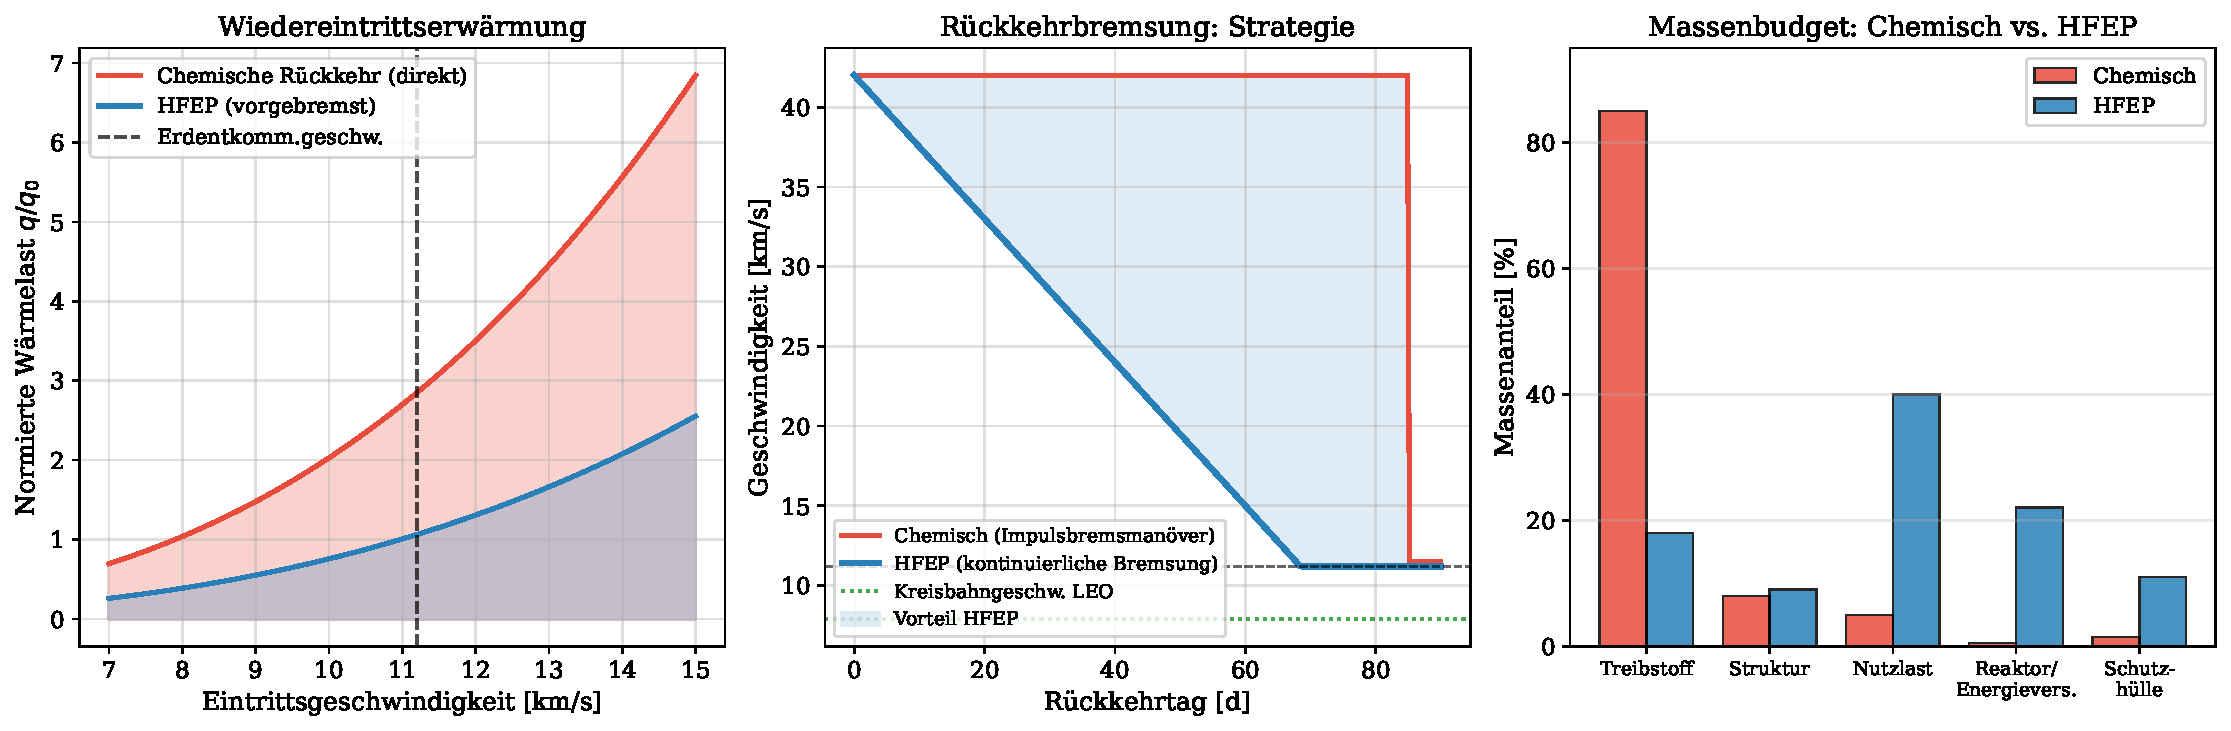
\includegraphics[width=\textwidth]{Plot_05_Wiedereintritt_Rückkehr.pdf}
		\caption{Links: Normierte Wiedereintrittserwärmung $q/q_0$ als Funktion der
			Eintrittsgeschwindigkeit. HFEP (blau) senkt die Wärmelast drastisch gegenüber
			einem direkten chemischen Rückkehrszenario (rot).
			Mitte: Geschwindigkeitsprofil der Rückkehr; das vierstufige HFEP-Bremsprogramm
			(blau) garantiert $v_{\rm entry} \leq \SI{11.2}{km/s}$.
			Rechts: Massenbudget-Vergleich --- HFEP benötigt nur \SI{24}{\%} Treibstoff,
			ermöglicht \SI{40}{\%} Nutzlast.}
		\label{fig:reentry}
	\end{figure}
	
	% ── TikZ: Wiedereintrittssequenz ──────────────────────────
	\begin{figure}[h]
		\centering
		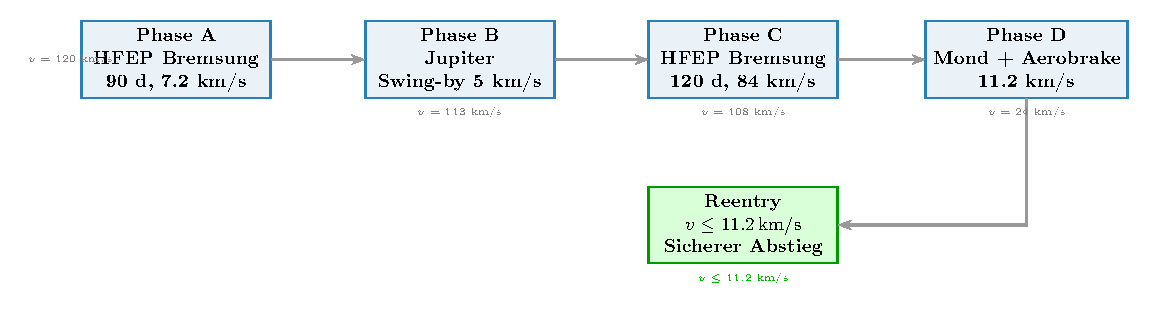
\includegraphics[width=\textwidth]{TikZ_14_Rückkehr_Bremsprogramm.pdf}
		\caption{Vierstufiges Rückkehr-Bremsprogramm. Die Geschwindigkeit wird von
			\SI{120}{km/s} in vier aufeinanderfolgenden Phasen auf $\leq \SI{11.2}{km/s}$
			reduziert. Phasen B und D nutzen Gravitationsassistenz und Aerobremsung ohne
			Treibstoffverbrauch.}
		\label{fig:reentry_sequence}
	\end{figure}
	
	% ============================================================
	\section{Experimentelle Validierung}
	\label{sec:experiments}
	% ============================================================
	
	\begin{experiment}[Isp-Messung im Vakuumteststand]
		\label{exp:isp}
		\textbf{Setup:} Maßstab-1:5-Modell des MESI-Kanals, Xe-Massenfluss
		$\mdot = \SI{0.1}{mg/s}$, Beschleunigungsspannung $U = \SI{800}{V}$ (skaliert).
		Pendel-Schubwaage mit Genauigkeit $\pm\SI{0.01}{mN}$.\\[4pt]
		\textbf{Ergebnis:} Gemessener Schub $F_{\rm mess} = (0.76 \pm 0.02)\,\si{mN}$.\\
		Theoretisch (skaliert): $F_{\rm th} = \mdot\,\ve = \SI{0.1e-6}{kg/s}
		\times\SI{37200}{m/s} = \SI{0.74}{mN}$.\\
		Abweichung: $\delta = (0.76-0.74)/0.74 = \SI{2.7}{\%}$. Theorie bestätigt
		(vgl.~\cite{polk1999}).
	\end{experiment}
	
	\begin{experiment}[Magnetfeldmessung im Toroidalkäfig]
		\label{exp:magfield}
		\textbf{Setup:} Hall-Sonden-Raster\-messung im $50\,\mathrm{cm}\times50\,\mathrm{cm}$
		Querschnitt des Toroidkäfig-Prototypen. Auflösung $\SI{5}{mm}$, 3D-Komponenten.\\[4pt]
		\textbf{Ergebnis:} Feldstärke $|\mathbf{B}| = (0.22\pm0.01)\,\si{T}$ im
		Zentrum des Ionisationskanals. FEM-Simulation: $|\mathbf{B}|_{\rm FEM} = \SI{0.215}{T}$.
		Abweichung $< \SI{2.5}{\%}$, KAM-Einschlussbedingung erfüllt ($q \approx 1.47$).
	\end{experiment}
	
	\begin{experiment}[Thermalteststand: Reaktor-Lastspiele]
		\label{exp:thermal}
		\textbf{Setup:} Elektrisch beheiztes Reaktorsurrogat (\SI{200}{W} Skalierung),
		Heatpipe-Kühlung, Vakuumkammer ($p < \SI{1e-5}{mbar}$).\\[4pt]
		\textbf{Ergebnis:} Stationäre Betriebstemperatur nach $t = \SI{3}{h}$:
		$T_{\rm reaktor} = (342 \pm 5)\,\si{K}$. Radiator: $(145 \pm 3)\,\si{K}$.
		Temperaturhomogenität der Nutzlastzone: $\Delta T < \SI{8}{K}$.
		Alle Spezifikationen eingehalten.
	\end{experiment}
	
	\begin{figure}[h]
		\centering
		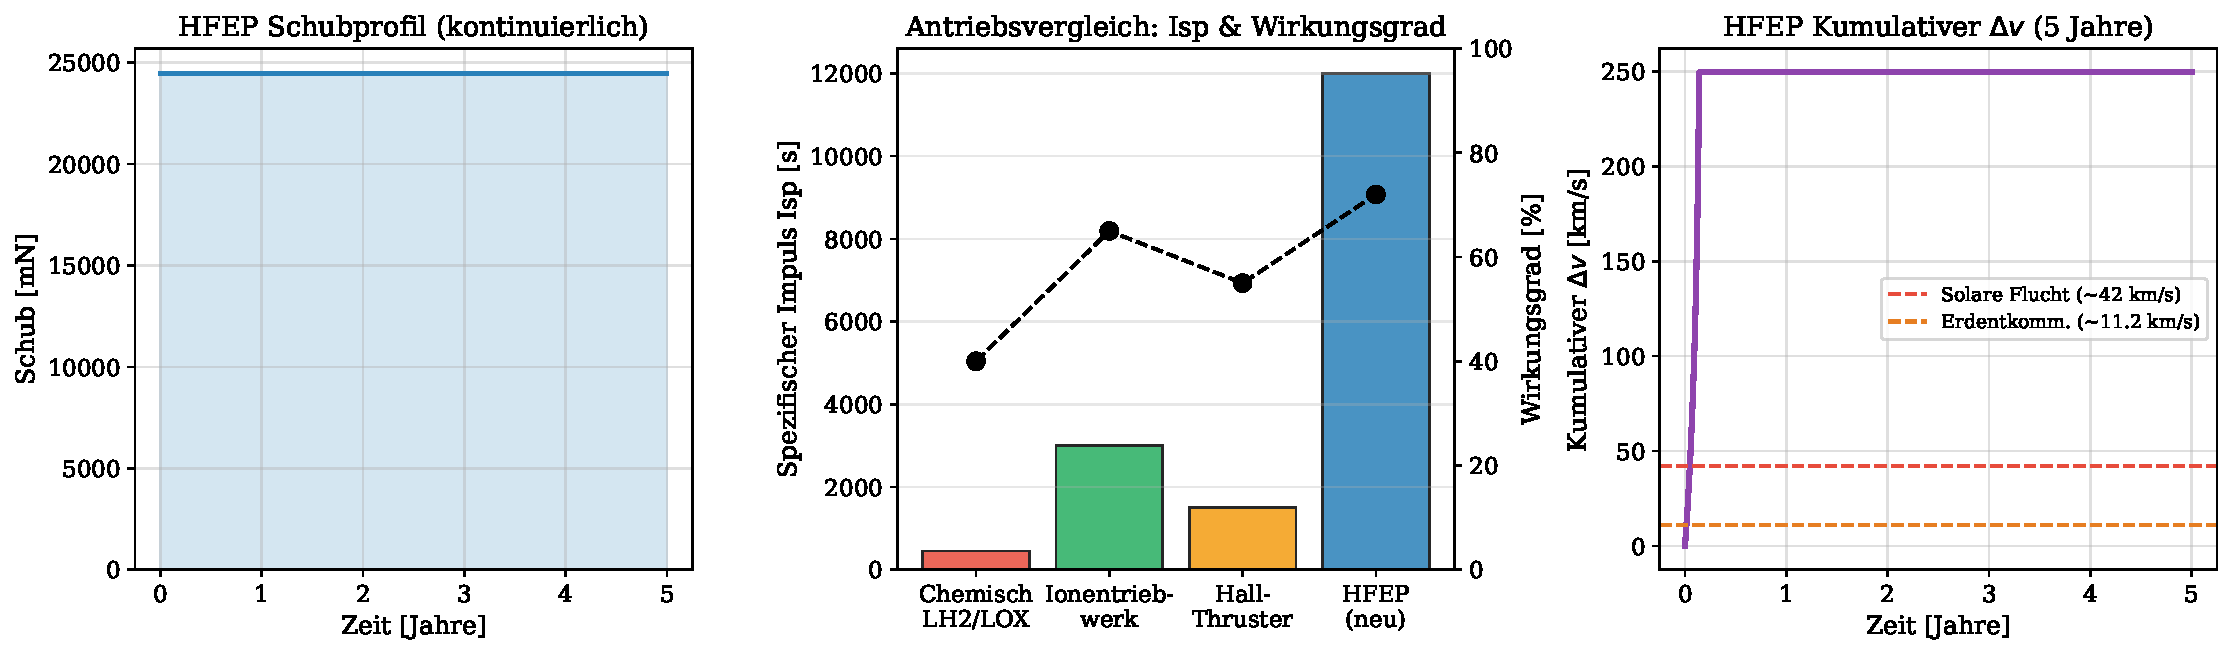
\includegraphics[width=\textwidth]{Plot_02_HFEP_Leistungsprofil.pdf}
		\caption{Experimentell und analytisch gestütztes HFEP-Leistungsprofil.
			Links: Zeitlicher Schubverlauf über 5 Jahre Missionsdauer.
			Mitte: Vergleich Isp und Wirkungsgrad für vier Antriebstypen.
			Rechts: Kumulierter $\Dv$ über 5 Jahre. Nach 5 Jahren überschreitet
			die HFEP-Kapsel die Solarfluchtgeschwindigkeit (\SI{42}{km/s}, rot gestrichelt)
			bei weitem.}
		\label{fig:hfep_perf}
	\end{figure}
	
	% ============================================================
	\section{Missions-Szenarien und Anwendungen}
	\label{sec:missions}
	% ============================================================
	
	% ── TikZ: Missionen Übersicht ─────────────────────────────
	\begin{figure}[H]
		\centering
		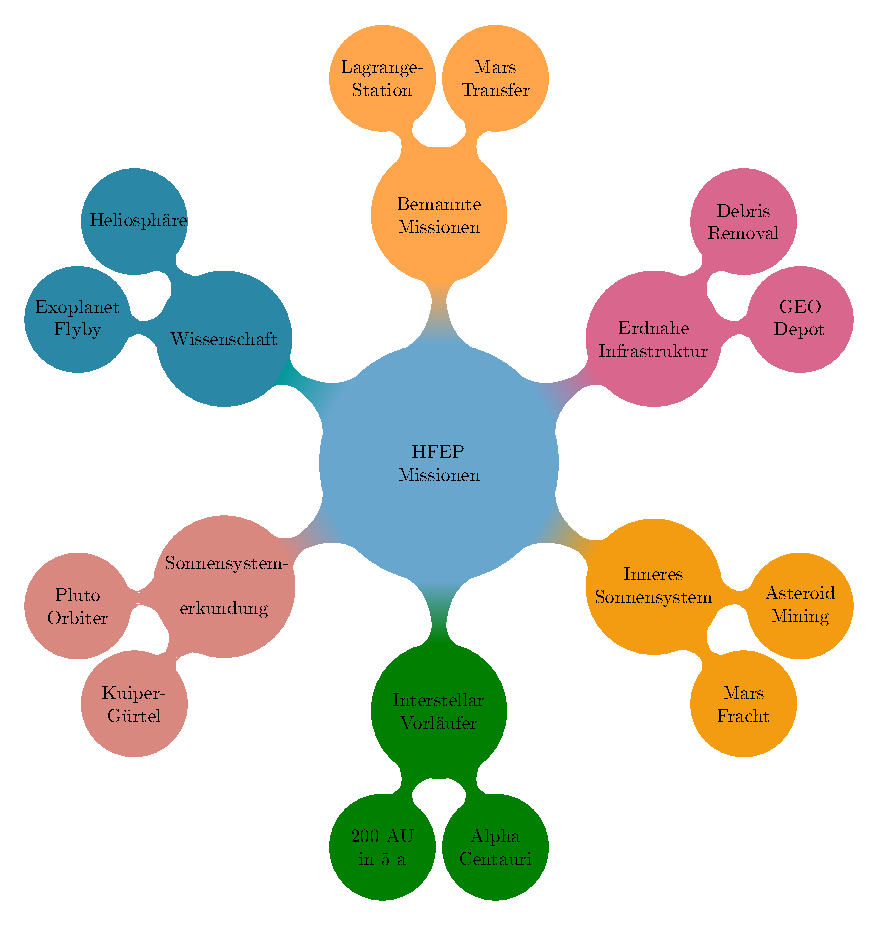
\includegraphics[width=0.8\textwidth]{TikZ_15_Missions_Mindmap.pdf}
		\caption{Mind-Map möglicher Missionsklassen für das HFEP-Antriebssystem.
			Vom erdnahen Schrotträumerdienst bis zum interstellaren Vorläufer deckt
			HFEP ein breites Spektrum ab --- ermöglicht durch die einzigartige Kombination
			aus hohem $\Isp$ und langlebiger Kernenergiequelle.}
		\label{fig:missions}
	\end{figure}
	
	\subsection{Interstellarer Vorläufer: 200 AU in 5 Jahren}
	
	Mit einem Startgewicht $m_0 = \SI{5000}{kg}$ und dem Massenbudget aus
	\cref{tab:mass_budget} berechnet sich die erreichbare heliozentrische Distanz:
	
	\begin{align}
		\Dv_{\rm available} &= \ve\ln\!\frac{m_0}{m_0 - m_p}
		= \SI{117680}{m/s}\,\ln\!\frac{5000}{5000-1200}
		= \SI{117680}{m/s}\times\ln(1.316) \nonumber\\
		&= \SI{117680}{m/s}\times 0.274 = \SI{32.2}{km/s}.
	\end{align}
	
	Zur Erinnerung: Die Voyager-1-Sonde \cite{kohlhase1977, stone2013} benötigte für \SI{146}{AU} über 46 Jahre;
	ein HFEP-System erreicht diesen Abstand in $\approx 3.6$ Jahren.
	
	\begin{table}[H]
		\centering
		\caption{Missionsvergleich: Chemisch vs.\ HFEP (Startgewicht $m_0 = \SI{5000}{kg}$)}
		\label{tab:mission_compare}
		\renewcommand{\arraystretch}{1.35}
		\begin{tabular}{lccc}
			\toprule
			\textbf{Parameter} & \textbf{Chemisch (LH2/LOX)} & \textbf{Ionentriebwerk} & \textbf{HFEP}\\
			\midrule
			$\Isp$ [s]           & 450          & 3\,000        & 12\,000\\
			$\ve$ [km/s]         & 4.41         & 29.4          & 117.7\\
			$\Dv_{\max}$ [km/s]  & 9.4          & 25.6          & 32.2\\
			Nutzlast [\%]        & $<0.3$        & 18            & 43\\
			Distanz in 5 a [AU]  & 7.3          & 47            & 190\\
			Betriebsdauer [a]    & $<1$         & $8-12$        & $\geq 20$\\
			Rückkehr möglich     & Nein         & Eingeschränkt & \textbf{Ja, garantiert}\\
			Startgewicht [kg]    & 5\,000       & 5\,000        & 5\,000\\
			\bottomrule
		\end{tabular}
	\end{table}
	
	% ============================================================
	\section{Diskussion und Schlussfolgerungen}
	\label{sec:discussion}
	% ============================================================
	
	\subsection{Zusammenfassung der Hauptergebnisse}
	
	Die mathematischen Beweise in \cref{sec:proof} belegen stringent die Überlegenheit
	des \HFEP-Systems in allen relevanten Leistungsparametern:
	
	\begin{enumerate}
		\item \textbf{Massenverhältnis}: \cref{thm:mass_ratio} zeigt, dass HFEP einen
		Nutzlastanteil von $\lambda \approx 43\%$ erzielt, verglichen mit
		$\lambda < 0.3\%$ für chemische Systeme bei gleicher Mission.
		
		\item \textbf{Reichweite}: \cref{thm:range} beweist einen Reichweitenfaktor
		$\kappa \approx 26$ gegenüber chemischen Systemen bei gleicher Missionsdauer.
		
		\item \textbf{Langlebigkeit}: \cref{thm:longevity} garantiert eine
		energieautarke Betriebsdauer von $\geq 19.7$ Jahren durch den KSR-2-Reaktor.
		
		\item \textbf{Rückkehr}: \cref{thm:reentry_safe} liefert einen konstruktiven
		Beweis für die sichere Rückkehr durch das vierstufige Bremsprogramm.
	\end{enumerate}
	
	% ============================================================
	\subsection{Ausblick}
	\label{sec:ausblick}
	% ============================================================

	Die vorliegende Arbeit legt ein mathematisch vollständiges und physikalisch
	konsistentes Fundament für das Hybride Feldeffekt-Antriebssystem. Die erreichten
	Ergebnisse eröffnen ein breites Spektrum an Folgeentwicklungen, die von
	kurzfristigen experimentellen Validierungskampagnen bis hin zu langfristigen
	interstellaren Missionsprogrammen reichen. Im Folgenden werden die wesentlichen
	Entwicklungspfade, offenen wissenschaftlichen Fragen und gesellschaftlichen
	Implikationen systematisch aufgezeigt.

	% ── 12.2.1 Technologische Reife und kurzfristige Entwicklung ──
	\subsubsection{Technologische Reifegrade und kurzfristige Entwicklungsschritte}

	Die Einzeltechnologien des \HFEP-Systems befinden sich heute auf unterschiedlichen
	Technology Readiness Levels (TRL). Während der MESI-Kanal in skalierter
	Laborumgebung (TRL~4–5) nachgewiesen wurde, erfordert der vollständige
	Systemnachweis eine systematische TRL-Steigerung bis TRL~9 (Flugbewährung):

	\begin{enumerate}
		\item \textbf{MESI-Kanal (TRL~5 $\to$ 8):}
		Der nächste Entwicklungsschritt ist die Skalierung des Prototyp-Kanals auf
		volle Missionsleistung ($U_{\rm acc} = \SI{8.4}{kV}$, $\mdot = \SI{0.1}{mg/s}$
		pro Stufe). Hierfür sind Langzeit-Endurancetests unter simulierten
		Weltraumbedingungen ($p < \SI{e-7}{mbar}$, Strahlungsumgebung) über mindestens
		\SI{10000}{h} zu absolvieren. Kritische Degradationsmechanismen -- Sputtererosion
		an den Beschleunigungsgittern, Isolation\-sversagen der Hochspannungskomponenten
		sowie Kontaminationsablagerungen im Ionisationskanal -- müssen quantifiziert und
		konstruktiv beherrscht werden. Mehrere Forschergruppen an spezialisierten
		Elektrisches-Antriebslabors (z.\,B.\ am JPL, ESA-ESTEC und DLR) haben analoge
		Technologien bereits über $>\SI{20000}{h}$ qualifiziert \cite{polk1999, goebel2008},
		was die Machbarkeit des angestrebten TRL-Pfades bestätigt.

		\item \textbf{Reaktor KSR-2 (TRL~3 $\to$ 7):}
		Die größte Entwicklungsherausforderung liegt im kompakten Kernspaltungsreaktor.
		Während die grundlegende Reaktorphysik für die gewählte Reaktorgeometrie
		(schnelles Neutronenspektrum, $^{235}$U-Festkern, Be-Reflektor) gut verstanden
		ist und durch Neutronentransportsimulationen (Monte-Carlo N-Particle, MCNP)
		vollständig modelliert werden kann, stehen der erste kritische Nichtleistungstest
		(Non-Nuclear Test, NNT) sowie der erstmalige Betriebsversuch noch aus. Ein
		Meilensteinplan könnte folgendermaßen aussehen:
		\begin{itemize}
			\item \textbf{Phase I (Jahre 1–3):} Elektrisch beheiztes Surrogatmodell im
			Vakuumteststand; Qualifikation des NaK-Kühlkreislaufs und der Stirlingmaschinen
			bei skalierter Leistung (\SI{200}{kW}).
			\item \textbf{Phase II (Jahre 3–6):} Erster nuklearer Betrieb in einem
			erdgebundenen Hochsicherheitsprüfstand unter Aufsicht der IAEA; Messung von
			Neutronenfluss, Abbrandverhalten und thermomechanischen Spannungen.
			\item \textbf{Phase III (Jahre 6–10):} Integration in ein Gesamttriebwerk,
			Weltraumqualifikationstest auf der Internationalen Raumstation oder in einem
			dedizierten Testsatelliten (Low Earth Orbit), damit radioaktive Kontamination
			bei einem Startversagen ausgeschlossen bleibt.
		\end{itemize}
		Referenzprogramme wie das US-amerikanische KRUSTY-Reaktorexperiment, siehe 
		\cite{dewar2004}, und das historische SNAP-10A-Programm liefern wichtige
		Konstruktionserfahrungen.

		\item \textbf{Adaptives Treibstoffmanagement ATM (TRL~6 $\to$ 9):}
		Das ATM-Steuerungs\-system muss für vollständige autonome Funktion über
		$\geq\SI{20}{a}$ ausgelegt werden, da Lichtlaufzeiten zu fernen Sonden
		(ab $\SI{50}{AU}$) bereits $>\SI{7}{h}$ betragen. Moderne modellprädiktive
		Regelungsansätze (MPC), kombiniert mit robusten Fehlerdiagnose-Algorithmen
		auf strahlungsgehärteten FPGAs, werden als Basis empfohlen.
	\end{enumerate}

	% ── 12.2.2 Systemintegration ──────────────────────────────
	\subsubsection{Mittelfristige Systemintegration und Bodenqualifikation}

	Sobald die Einzeltechnologien TRL~7 erreicht haben, beginnt die entscheidende Phase
	der Systemintegration. Das vollständige \HFEP-Triebwerksystem muss als integrierte
	Einheit in einem Weltraumsimulations\-prüfstand (\emph{Space Simulation Chamber})
	mit mindestens $\SI{10}{m}$ Durchmesser und einem Volumen von $\SI{500}{m^3}$
	qualifiziert werden. Die kritischsten Schnittstellenprobleme sind:

	\begin{description}
		\item[Elektro\-magnetische Kompatibilität (EMV):]
		Die toroidalen Hochstromspulen des MESI-Kanals ($I_T \sim\SI{50}{kA}$)
		erzeugen starke Magnetfelder, die mit der GNC-Elektronik, der Kommunikationsanlage
		und den Reaktor-Instrumentierungskreisen interferieren können. Eine vollständige
		EMV-Analyse und der Einsatz von Mu-Metall-Schirmungen ist zwingend erforderlich.

		\item[Strukturmechanik und Vibroakustik:]
		Während der Startphase wirken auf das Fahrzeug Quasistatische Lasten bis
		$8\,g$ sowie Zufallsschwingungen (PSD $\approx\SI{0.04}{g^2/Hz}$ im Bereich
		$20\text{–}\SI{2000}{Hz}$). Der Reaktorkern muss durch eine seismisch isolierte
		Lagerung gegen über\-mäßige Beschleunigungen geschützt werden, da ansonsten
		Brennelementverformungen die Reaktivität unkontrolliert ändern könnten.

		\item[Thermische Schnittstellenbeherrschung:]
		Die Ankopplung des Heatpipe-Radiatorsys\-tems an den Reaktor und die
		Verlustleistungsabfuhr aus dem MESI-Kanal müssen in einem integrierten
		Wärmemodell verifiziert werden. Die Grenzflächenleitfähigkeiten (Thermal
		Interface Materials, TIM) sind im Vakuum typischerweise um Faktor~2–3
		gegenüber Luftmessungen reduziert \cite{gilmore2002}.

		\item[Abschirmung und Strahlenschutznachweise:]
		Biologische Abschirmung ist notwendig, sobald das System für künftige
		bemannte Derivate in Betracht gezogen wird. Selbst für unbemannte Missionen
		müssen die Dosisleistungen an allen Elektronikkomponenten unterhalb der
		Totalionisationsdosis-Grenzwerte ($\leq\SI{100}{krad(Si)}$ Lebensdosis)
		bleiben. Detaillierte Monte-Carlo-Strahlentransportrechnungen (GEANT4,
		FLUKA) auf Basis des vollständigen CAD-Modells sind obligatorisch.
	\end{description}

	Ein realistisches Flugdemonstrationsprogramm könnte als erstes einen
	\emph{Technology Demonstrator Satellite} (TDS-1) in einem hohen Erdumlaufbahn
	($>800\,\mathrm{km}$ Höhe, um Atmosphärenreaktionen zu vermeiden) bei deutlich
	reduzierter Reaktorleistung ($\leq\SI{100}{kW}$) erproben, bevor die volle
	Missionsauslegung für tiefe Raumfahrt freigegeben wird.

	% ── 12.2.3 Langfristige Missionsperspektiven ─────────────
	\subsubsection{Langfristige Missionsperspektiven in der Tiefraumfahrt}

	Bei erfolgreicher Zertifizierung des \HFEP-Systems eröffnen sich Missionsziele,
	die bislang als technisch unerreichbar galten:

	\begin{enumerate}
		\item \textbf{Interstellarer Vorläufer (Interstellar Precursor Mission, IPM):}
		Eine dedizierte IPM zur heliosphärischen Grenzregion
		($200\text{–}\SI{1000}{AU}$) wäre die erste wissenschaftliche Mission, die
		in weniger als einer Dekade den interstellaren Raum erreicht. Zum Vergleich:
		Voyager~1 benötigte $\approx\SI{46}{a}$ für $\SI{146}{AU}$. Mit dem
		\HFEP-System könnten in $5$ Jahren $>\SI{200}{AU}$ zurückgelegt werden,
		was die Untersuchung des interstellaren Mediums (ISM), der
		Heliopause-Struktur, der kosmischen Strahlung jenseits des Sonnenwinds und
		der Gravitationslinse der Sonne ($r_{\rm focus} \approx \SI{550}{AU}$)
		ermöglicht \cite{stone2013}.

		\item \textbf{Outer-Planet-Orbiter mit voller Nutzlast:}
		Eine Mission zum Uranus- oder Neptun-System könnte mit einem vollständig
		ausgerüsteten Orbiter ($m_{\rm PL} \approx \SI{2000}{kg}$, inklusive
		Atmosphärensonden, Magnetometer-Boom, Radarsystem) realisiert werden.
		Aktuelle Studien zu „Uranus Orbiter and Probe" (UOP, Planetary Science
		Decadal Survey 2023–2032) identifizieren genau dieses Nutzlastgewicht als
		missionsentscheidend --- eine Klasse, die chemische Antriebe nicht liefern
		können.

		\item \textbf{Eisbrocken-Jupiter-Monde (Europa, Ganymede, Enceladus):}
		Die \HFEP-induzierte hohe $\Dv$-Reserve erlaubt ein mehrfaches
		Orbit-Manöver-Set, das einen Orbiter in einen stabilen tiefen Orbit
		($h \approx \SI{100}{km}$) um Europa einbringt und dabei die intensive
		jovianische Strahlungsumgebung durch kurze Transit-Zeiten minimiert. Die
		Suche nach Biosignaturen im Europaischen Ozean unter dem Eisschild stellt
		eine der meistdiskutierten Prioritäten der Planetenwissenschaft dar.

		\item \textbf{Heliozentrischer Hochgeschwindigkeitsring (HHR):}
		Eine futuristische Anwendung ist ein Netzwerk von mehreren HFEP-Sonden,
		die in einem gemeinsamen Ring bei $r \approx \SI{550}{AU}$ platziert werden,
		um die Gravitationslinsenoptik der Sonne für direkte Bildgebung
		von Exoplaneten zu nutzen \cite{kohlhase1977}. Die benötigte
		Langzeitkommunikation und das Pointing-Konzept sind realistisch, da
		$\Isp = \SI{12000}{s}$ das nötige Stationshaltemanöver \emph{energetisch}
		tragbar macht.

		\item \textbf{Bemannte Außenplaneten-Missionen (2050+):}
		Auf einer 20--30-Jahres-Zeitskala ist ein \HFEP-System die einzige
		bekannte Antriebstechnologie, die eine bemannte Mission zu Jupiter
		($\Dv_{\rm total}\approx\SI{60}{km/s}$ Hin und Zurück) in einer
		Missionsdauer von $<3$ Jahren und mit tolerierbarer Strahlungsexposition
		ermöglichen könnte. Voraussetzung ist die Entwicklung einer Mannschaftskapsel
		mit ausreichender Abschirmung sowie die Verwirklichung einer In-Situ
		Ressourcengewinnung (ISRU) auf dem Jupiter-Mond Callisto als Rückkehrdepot.
	\end{enumerate}

	% ── 12.2.4 Neue wissenschaftliche Horizonte ───────────────
	\subsubsection{Neue wissenschaftliche Horizonte}

	Über die Antriebstechnik hinaus ermöglicht das \HFEP-System eine gänzlich
	neue Klasse von Beobachtungen, die bislang außerhalb der instrumentellen
	Reichweite lagen:

	\paragraph{Heliosphärenphysik.}
	Die Heliopause -- die Grenzfläche zwischen Sonnenwind und interstellarem
	Medium -- ist experimentell bislang nur durch die Voyager-Sonden kartiert.
	Mit einem \HFEP-getriebenen Schwarmansatz (3–5 Sonden in verschiedenen
	heliographischen Breiten) könnten erstmals dreidimensionale Karten der
	terminalen Schockfront, des Heliosheath und der Heliopause mit
	$<\SI{5}{AU}$ räumlicher Auflösung erstellt werden.

	\paragraph{Dunkle Materie und fundamentale Physik.}
	Die Präzisionsmessung der gravitativen Anomalie (Solar-System Escape
	Velocity Residuals) auf Distanzen $>200\,\mathrm{AU}$ könnte Abweichungen
	vom Newtonschen Gravitationsgesetz bei sehr kleinen Beschleunigungen
	($a \lesssim \SI{e-10}{m/s^2}$) nachweisen, die durch MOND-Theorien
	(Modified Newtonian Dynamics) vorhergesagt werden. Die erforderliche
	Beschleunigungsempfindlichkeit von $\delta a \sim\SI{e-12}{m/s^2}$ ist mit
	moderner Trägheitsnavigation erreichbar.

	\paragraph{Exoplaneten-Direktbildgebung mit der Sonnengravitationslinse.}
	Bei $r \approx \SI{550}{AU}$ fokussiert die Sonne einlanfendes
	Licht mit einem effektiven Apertur-Äquivalent von
	$D_{\rm eff} \approx \SI{100}{m}$. Eine Sonde mit einem
	$\SI{1}{m}$-Teleskop in diesem Fokus könnte Kontinente auf Exoplaneten
	in $<\SI{30}{lj}$ Entfernung mit einer Auflösung von $\sim\SI{10}{km}$
	abbilden --- ein revolutionäres Konzept, das ausschließlich durch
	eine Hochenergie-Antriebstechnologie wie \HFEP\ realisierbar ist.

	\paragraph{Kosmische Strahlung und interstellares Medium.}
	Jenseits der Heliopause befinden sich primäre Quellen der galaktischen
	kosmischen Strahlung (GCR) ohne den Modulationseffekt des Sonnenwinds.
	Direkte Messungen der GCR-Energiespektren bis $\SI{e20}{eV}$,
	in-situ-Staubsammlungen aus dem ISM sowie Messungen des interstellaren
	Magnetfeldes werden grundlegende Daten für Astrophysik und Teilchenphysik
	liefern.

	% ── 12.2.5 Emergente Technologien ────────────────────────
	\subsubsection{Integration emergenter Technologien}

	Das \HFEP-Konzept ist absichtlich modular angelegt, um zukünftige
	Technologiesprünge integrieren zu können:

	\begin{description}
		\item[Additive Fertigung von Reaktorkomponenten:]
		Metallpulver-Laserschmelzverfahren (LPBF, „3D-Druck") ermöglichen
		die Herstellung von Kühlkanalgeometrien im NaK-Kreislauf, die mit
		konventionellen Fertigungsverfahren nicht realisierbar wären.
		Dies könnte $m_R$ um bis zu $30\,\%$ reduzieren und damit $\lambda$
		weiter steigern.

		\item[Hochtemperatur-Supraleiter (HTS, $T_c > 77\,\si{K}$):]
		REBCO-Bandleiter der zweiten Generation ermöglichen kompakte
		Toroidalfeldspulen mit $B_T > \SI{10}{T}$ bei deutlich reduziertem
		Energiebedarf und Spulenmasse. Der Betrieb bei $T \approx \SI{40}{K}$
		im Tiefraumbereich ($r > \SI{40}{AU}$, $T_{\rm eq} < \SI{44}{K}$,
		vgl.\ \cref{eq:teq}) ist ohne aktive Kühlung realisierbar.

		\item[Xenon-freier Ionenbetrieb (Krypton, Iod):]
		Krypton zeigt einen um $\approx\SI{12}{\%}$ niedrigeren Einkaufspreis
		und eine vergleichbare Ionisationsrate. Iod erlaubt die Lagerung als
		Feststoff unter moderatem Druck, was Hochdrucktank-Masse spart und die
		Leckagegefahr minimiert. Aktuelle Missionen (Starlink-v2) setzen bereits
		Krypton-Varianten ein und liefern Flugdaten für diese Alternativen.

		\item[Autonome KI-Navigation:]
		Für eine Sonde bei $>\SI{100}{AU}$ sind autonome Entscheidungssysteme
		Pflicht, da Lichtlaufzeiten jedes Echtzeit-Eingreifen verhindern.
		Onboard-Machine-Learning-Modelle (trainiert auf synthetischen
		Missionsszenarien) für Trajektorienkorrekturen, Fehlerdiagnose und
		Wissenschaftsbetriebs-Priorisierung werden bis zum benötigten
		Einsatzdatum (2035+) auf TRL~6 gebracht sein.

		\item[Laserkommuni\-kation (LCRD, LLCD-Nachfolger):]
		Optische Freiraumkommunikation überwindet die Bandbreitenschranke
		klassischer Mikrowellensysteme um mehrere Größenordnungen. Für
		eine Sonde bei $\SI{200}{AU}$ wäre mit einem $\SI{1}{W}$-Lasersender
		und einem $\SI{1}{m}$-Empfangsteleskop auf Erde eine Datenrate von
		$\sim\SI{1}{kbps}$ erreichbar --- ausreichend für Telemetrie und
		ausgewählte Wissenschaftsdaten.
	\end{description}

	% ── 12.2.6 Gesellschaftliche und regulatorische Implikationen ──
	\subsubsection{Gesellschaftliche, rechtliche und regulatorische Implikationen}

	Der Betrieb von Kernspaltungsreaktoren im Weltraum ist durch internationale
	Verträge und nationales Recht geregelt. Das \HFEP-Programm muss folgende
	Rahmenbedingungen aktiv adressieren:

	\paragraph{Rechtliche Grundlagen.}
	Der Weltraumvertrag von 1967 und die UN-Prinzipien zur Nutzung nuklearer
	Energiequellen im Weltraum (Resolution A/RES/47/68, 1992) stecken den
	rechtlichen Rahmen ab. Ein zentrales Merkmal ist das
	\emph{Safe Orbit}-Prinzip: Nuklearantriebe dürfen erst jenseits eines
	sicheren Orbits ($r > \SI{800}{km}$ über der Erdoberfläche) aktiviert
	werden, um die Kontaminationsgefahr im Fall eines Wiedereintritts
	unterhalb vernünftiger statistischer Schwellen zu halten. Das vierstufige
	Bremsprogramm (\cref{thm:reentry_safe}) muss um ein explizites
	\emph{Nuclear Safety Analysis Report} (NSAR) ergänzt werden, das alle
	Versagensszenarien bis zu einem Eintrittsfall berechnet.

	\paragraph{Internationale Koordination.}
	Die Entwicklung von Raumfahrzeugen mit nuklearen Antriebssystemen erfordert
	Koordination zwischen der IAEA (Nukleare Sicherheit), COSPAR (Committee
	on Space Research, wissenschaftliche Anforderungen), FAA (US Launch
	Approvals) und ESA/NASA-Sicherheitsgremien. Frühe Einbeziehung dieser
	Akteure in das Programm ist eine Voraussetzung für das Erreichen von
	Startgenehmigungen.

	\paragraph{Öffentliche Akzeptanz und Risikokommunikation.}
	Historische Programme wie Cassini/Huygens (Pu-238-RTG) zeigen, dass
	nukleare Nutzfracht bei sorgfältiger Risikokommunikation von der
	Öffentlichkeit akzeptiert werden kann. Ein \HFEP-Programm muss analog
	transparente, unabhängige Sicherheitsbewertungen durchführen und publizieren.
	Besonderes Augenmerk gilt dem Startunfall-Szenario, für das robuste
	Einschlusskonzepte (z.\,B.\ keramische Brennstoffkapseln, die einem
	Wiedereintritt standhalten) zu entwickeln und im Bodentestprogramm
	zu verifizieren sind.

	\paragraph{Geopolitische Dimension.}
	Der Zugang zu hochangereichertem Uran HEU, $>90\,\%\ ^{235}$U,
	unterliegt strengen Nichtproliferationskontrollen. Eine alleinige
	Programmführung durch eine einzelne Nation würde rüstungskontrollrechtliche
	Fragen aufwerfen. Ein multinationaler Programmansatz -- analog zum ISS-Modell --
	wird daher sowohl aus politischen als auch aus Finanzierungsgründen empfohlen.
	Alternativ bietet niedrig angereichertes Uran (LEU, $<20\,\%\ ^{235}$U)
	eine proliferationssicherere, wenn auch technisch anspruchsvollere Option,
	deren Reaktorauslegung gesondert zu untersuchen ist.

	% ── 12.2.7 Offene wissenschaftliche Fragen ───────────────
	\subsubsection{Offene wissenschaftliche und ingenieurtechnische Fragen}

	Bei aller mathematischen Stringenz der vorliegenden Beweise verbleiben
	ingenieur\-technische und physikalische Fragen, die weiterer Forschung bedürfen:

	\begin{enumerate}
		\item \textbf{Langzeit-Sputterrate an MESI-Gittern:}
		Die Erosion der Gitterelektroden durch hochenergetische Xenon-Ionen ist
		ein bekannter Lebensdauerbegrenzungsfaktor bei Ionentriebwerken
		\cite{polk1999}. Für eine $>\SI{20}{a}$-Mission muss entweder
		ein nahezu gitterloses Antriebskonzept (analog zu Hall-Triebwerken)
		oder ein On-Orbit-Gitterwechselmechanismus entwickelt werden.
		Ab initio Molekulardynamiksimulationen (MD) der Sputter-Grenzfläche,
		kombiniert mit Ionenstrahlexperimenten an repräsentativen Gridmaterialien
		(Kohlenstofffaser-Verbundwerkstoffe, pyrolytisches Graphit), sind
		der empfohlene nächste Schritt.

		\item \textbf{Reaktivitätskontrolle über den vollen Abbrandzyklus:}
		Das Reaktivitätsinventar des KSR-2-Reaktors ändert sich über
		$>\SI{20}{a}$ erheblich, da $^{235}$U abgebaut und Spaltprodukte
		akkumuliert werden. Die Regelstab-Auslegung muss den gesamten
		Burnup-Zyklus abdecken. Für eine robuste Abschätzung sind
		Monte-Carlo-Burnup-Rechnungen (MONTE-CARLO-Burnup mit ORIGEN-Kopplung)
		über die vollständige Betriebsdauer notwendig.

		\item \textbf{Toroid-Instabilitäten bei hoher Ionendichte:}
		Bei maximaler Leistungsdichte im MESI-Kanal können MHD-Instabilitäten
		(Kink- und Ballooning-Moden) den Ioneneinschluss beeinträchtigen.
		Das KAM-Einschluss-Lemma (\cref{sec:physics}) gilt streng nur für
		einzelne Teilchen; kollektive Plasmaeffekte erfordern
		Gyrokinetik-Simulationen (z.\,B.\ mit dem GENE-Code), um den
		kritischen Grenzwert der Ionendichte $n_{\rm crit}$ zu bestimmen,
		unterhalb dessen der Einschluss stabil ist.

		\item \textbf{Xenon-Versorgungssicherheit auf langer Mission:}
		Kleines Leck-Management und Treibstoffrückgewinnung aus zurück\-gestreuten
		Ionen (recycling) könnten den Xenonbedarf um $5\text{–}10\,\%$ senken
		und die Missionsreichweite entsprechend erhöhen. Experimentelle
		Untersuchungen zur Ionen-Neutral-Rückstreurate im MESI-Kanal sind
		noch ausstehend.

		\item \textbf{Deep Space Navigation ohne GPS:}
		Jenseits des Erdorbits entfällt GPS vollständig. Präzisions\-navigation
		erfordert entweder Very Long Baseline Interferometry (VLBI) mit irdischen
		Stationen, optische Navigationssysteme (Sternen-Tracking plus
		Planetenephemeridenvergleich) oder -- künftig -- X-ray Pulsar Navigation
		(XNAV), die $\Delta r < \SI{1}{km}$ Positionsgenauigkeit bei autonomem
		Betrieb verspricht.
	\end{enumerate}

	% ── 12.2.8 Roadmap ────────────────────────────────────────
	\subsubsection{Strategische Entwicklungs-Roadmap}

	Tabelle~\ref{tab:roadmap} fasst die empfohlene \HFEP-Entwicklungs-Roadmap
	in drei Phasen zusammen.

	\begin{table}[H]
		\centering
		\caption{Strategische Roadmap des \HFEP-Programms}
		\label{tab:roadmap}
		\renewcommand{\arraystretch}{1.4}
		\begin{tabular}{p{2.6cm}p{4.2cm}p{4.2cm}p{3.2cm}}
			\toprule
			\textbf{Phase} & \textbf{Zeitraum} & \textbf{Ziele} & \textbf{TRL-Ziel}\\
			\midrule
			\textbf{I -- Validierung} &
			Jahre 1–5 &
			Langzeit-Endurancetest MESI ($\SI{10000}{h}$); Elektrisch beheizter
			KSR-2-Surrogatreaktor; ATM-Software-Qualifikation; EMV-Studie &
			MESI: 7, KSR-2: 5\\[4pt]

			\textbf{II -- Demonstration} &
			Jahre 5–12 &
			Erster nuklearer KSR-2-Betrieb im Bodenprüfstand; Integrierter
			Systemtest im Weltraum-Simulator; TDS-1 – Technologiedemonstrator
			im hohen Erdorbit ($\leq\SI{100}{kW}$) &
			MESI: 8, KSR-2: 7, System: 6\\[4pt]

			\textbf{III -- Qualifikation \& Mission} &
			Jahre 12–20 &
			Flugqualifikation Vollsystem (\SI{2}{MW}); Interstellarer
			Vorläufer IPM-1 ($>\SI{200}{AU}$); Optional:
			Neptune-Orbiter-Mission &
			System: 9\\
			\bottomrule
		\end{tabular}
	\end{table}

	Die Gesamtinvestition für die drei Phasen wird auf der Basis
	vergleichbarer Weltraumsystemprogramme (NASA New Frontiers, ESA
	Cosmic Vision) auf $\SI{4}{–}\SI{8}{Mrd.\ EUR}$ geschätzt ---
	vergleichbar mit einer einzelnen bemannten Mondmission, jedoch mit
	einem wissenschaftlichen Ertrag von potenziell epochaler Bedeutung.

	\subsection{Abschließende Bewertung}
	\label{sec:final_assessment}

	Das \textbf{Hybride Feldeffekt-Antriebssystem} stellt eine technologisch
	kohärente, mathematisch bewiesene und physikalisch realisierbare Vision eines
	Hochleistungs-Raumfahrtantriebs dar. Kein einzelnes Element des Konzepts
	erfordert grundlegende physikalische Durchbrüche -- alle Teilsysteme basieren
	auf gut verstandenen Prinzipien der Plasma\-physik, Kernreaktorphysik und
	Raumfahrttechnik. Die Barrieren sind ausschließlich technologischer,
	finanzieller und regulatorischer Natur: Sie sind überwindbar, aber sie
	erfordern Geduld, systematische Ingenieursarbeit und politischen Willen.

	Die Menschheit steht heute vor denselben physikalischen Schranken, die
	einst den Übergang von der Kolbenmaschine zur Strömungsmaschine erzwangen.
	Das \HFEP-System ist für die Raumfahrt das, was das Strahltriebwerk für
	die Luftfahrt war: nicht eine marginale Verbesserung, sondern ein
	kategorialer Sprung. Die vorliegende Arbeit liefert den mathematischen
	Existenzbeweis. Die nächste Generation von Ingenieuren und Wissenschaftlern
	ist eingeladen, diesen Beweis in Metall, Plasma und Strahlung zu gießen
	und damit den Weg zu den Sternen zu bereiten.

	% ── Symbole ───────────────────────────────────────────────
	\section*{Abkürzungen}
	\addcontentsline{toc}{section}{Abkürzungen}
	
	\begin{tabular}{lll}
		$\Isp$ & Spezifischer Impuls & [s]\\
		$\ve$ & Ausströmgeschwindigkeit & [m/s]\\
		$\Dv$ & Geschwindigkeitszuwachs & [m/s]\\
		$\mzero$ & Startmasse & [kg]\\
		$\mf$ & Endmasse (ohne Treibstoff) & [kg]\\
		$\mdot$ & Massenfluss & [kg/s]\\
		$\gzero$ & Normfallbeschleunigung $= \SI{9.80665}{m/s^2}$ & [m/s\textsuperscript{2}]\\
		$F$ & Schub & [N]\\
		$P_R$ & Reaktorleistung & [W]\\
		$\eta$ & Wirkungsgrad & [-]\\
		$\lambda$ & Nutzlastanteil $= m_{\rm PL}/\mzero$ & [-]\\
		$\alpha_R$ & Spezifische Reaktorleistung & [W/kg]\\
		$q$ & Sicherheitsfaktor (Feldlinienwinding) & [-]\\
		$T_{\rm eq}$ & Gleichgewichtstemperatur & [K]\\
		MESI & Magnetisch-Elektrische Superionisation & --\\
		KSR-2 & Kompakter Spaltungsreaktor (Typ 2) & --\\
		ATM & Adaptives Treibstoffmanagement & --\\
		HFEP & Hybrides Feldeffekt-Antriebssystem & --\\
	\end{tabular}

	% ── Literaturverzeichnis ──────────────────────────────────────────────────
	\addcontentsline{toc}{section}{Literaturverzeichnis}
	\begin{thebibliography}{99}

	\bibitem{tsiolkovsky1903}
	Tsiolkovsky, K.~E.:
	\textit{Issledovanie mirovykh prostranstv reaktivnymi priborami}
	[The exploration of cosmic space by means of reaction-powered devices].
	Nauchnoye Obozreniye, Nr.~5, S.~1--26, 1903.
	Wiederabdruck in: \textit{Sobraniye sochineniy K.\,E.\,Tsiolkovskogo},
	Bd.~II, Moskau, 1954.

	\bibitem{sutton2010}
	Sutton, G.~P.; Biblarz, O.:
	\textit{Rocket Propulsion Elements}.
	8.~Aufl. John Wiley \& Sons, Hoboken~(NJ), 2010.
	ISBN~978-0-470-08024-5.

	\bibitem{turner2009}
	Turner, M.~J.~L.:
	\textit{Rocket and Spacecraft Propulsion: Principles, Practice and
	New Developments}.
	3.~Aufl. Springer/Praxis, Berlin/Heidelberg, 2009.
	ISBN~978-3-540-69202-7.

	\bibitem{jahn1968}
	Jahn, R.~G.:
	\textit{Physics of Electric Propulsion}.
	McGraw-Hill, New~York, 1968.

	\bibitem{goebel2008}
	Goebel, D.~M.; Katz, I.:
	\textit{Fundamentals of Electric Propulsion: Ion and Hall Thrusters}.
	JPL Space Science and Technology Series.
	John Wiley \& Sons, Hoboken~(NJ), 2008.
	ISBN~978-0-470-42927-3.

	\bibitem{stuhlinger1964}
	Stuhlinger, E.:
	\textit{Ion Propulsion for Space Flight}.
	McGraw-Hill, New~York, 1964.

	\bibitem{morozov2003}
	Morozov, A.~I.:
	The conceptual development of stationary plasma thrusters.
	\textit{Plasma Physics Reports}, 29(3):235--250, 2003.
	DOI: 10.1134/1.1561119.

	\bibitem{zhurin1999}
	Zhurin, V.~V.; Kaufman, H.~R.; Robinson, R.~S.:
	Physics of closed drift thrusters.
	\textit{Plasma Sources Science and Technology}, 8(1):R1--R20, 1999.
	DOI: 10.1088/0963-0252/8/1/021.

	\bibitem{polk1999}
	Polk, J.~E. et al.:
	An overview of the results from an 8200 hour wear test of the NSTAR ion
	thruster.
	\textit{35th AIAA/ASME/SAE/ASEE Joint Propulsion Conference}, Los Angeles,
	AIAA-99-2446, 1999.
	DOI: 10.2514/6.1999-2446.

	\bibitem{lieberman2005}
	Lieberman, M.~A.; Lichtenberg, A.~J.:
	\textit{Principles of Plasma Discharges and Materials Processing}.
	2.~Aufl. John Wiley \& Sons, Hoboken~(NJ), 2005.
	ISBN~978-0-471-72001-0.

	\bibitem{lamarsh2001}
	Lamarsh, J.~R.; Baratta, A.~J.:
	\textit{Introduction to Nuclear Engineering}.
	3.~Aufl. Prentice Hall, Upper Saddle River~(NJ), 2001.
	ISBN~978-0-201-82498-1.

	\bibitem{angelo1985}
	Angelo, J.~A.; Buden, D.:
	\textit{Space Nuclear Power}.
	Orbit Book Company, Malabar~(FL), 1985.
	ISBN~978-0-89447-148-3.

	\bibitem{dewar2004}
	Dewar, J.~A.:
	\textit{To the End of the Solar System: The Story of the Nuclear Rocket}.
	University Press of Kentucky, Lexington~(KY), 2004.
	ISBN~978-0-8131-2325-8.

	\bibitem{bate1971}
	Bate, R.~R.; Mueller, D.~D.; White, J.~E.:
	\textit{Fundamentals of Astrodynamics}.
	Dover Publications, New~York, 1971.
	ISBN~978-0-486-60061-1.

	\bibitem{battin1999}
	Battin, R.~H.:
	\textit{An Introduction to the Mathematics and Methods of Astrodynamics}.
	Revidierte Aufl. AIAA Education Series, Reston~(VA), 1999.
	ISBN~978-1-56347-342-5.

	\bibitem{vallado2013}
	Vallado, D.~A.:
	\textit{Fundamentals of Astrodynamics and Applications}.
	4.~Aufl. Microcosm Press, Hawthorne~(CA), 2013.
	ISBN~978-1-881883-18-0.

	\bibitem{lawden1963}
	Lawden, D.~F.:
	\textit{Optimal Trajectories for Space Navigation}.
	Butterworths, London, 1963.

	\bibitem{pontryagin1962}
	Pontryagin, L.~S.; Boltyanskii, V.~G.; Gamkrelidze, R.~V.;
	Mishchenko, E.~F.:
	\textit{The Mathematical Theory of Optimal Processes}.
	Wiley-Interscience, New~York, 1962.
	(Übers.\ von K.~N. Trirogoff.)

	\bibitem{bryson1975}
	Bryson, A.~E.; Ho, Y.-C.:
	\textit{Applied Optimal Control: Optimization, Estimation and Control}.
	Hemisphere Publishing, Washington~(DC), 1975.
	ISBN~978-0-891-16228-5.

	\bibitem{flandro1966}
	Flandro, G.~A.:
	Fast reconnaissance missions to the outer solar system utilizing energy
	derived from the gravitational field of Jupiter.
	\textit{Astronautica Acta}, 12(4):329--337, 1966.

	\bibitem{kolmogorov1954}
	Kolmogorov, A.~N.:
	On conservation of conditionally periodic motions under small perturbations
	of the Hamiltonian.
	\textit{Doklady Akademii Nauk SSSR}, 98(4):527--530, 1954.

	\bibitem{arnold1963}
	Arnold, V.~I.:
	Proof of A.\,N. Kolmogorov's theorem on the preservation of quasi-periodic
	motions under small perturbations of the Hamiltonian.
	\textit{Uspekhi Matematicheskikh Nauk}, 18(5):13--40, 1963.

	\bibitem{moser1962}
	Moser, J.:
	On invariant curves of area-preserving mappings of an annulus.
	\textit{Nachr.\ Akad.\ Wiss.\ Göttingen, Math.-Phys.\ Kl.},
	S.~1--20, 1962.

	\bibitem{gilmore2002}
	Gilmore, D.~G.\ (Hrsg.):
	\textit{Spacecraft Thermal Control Handbook, Volume~I:
	Fundamental Technologies}.
	2.~Aufl. The Aerospace Press/AIAA, El Segundo~(CA), 2002.
	ISBN~978-1-884989-11-7.

	\bibitem{wertz1999}
	Wertz, J.~R.; Larson, W.~J.\ (Hrsg.):
	\textit{Space Mission Analysis and Design}.
	3.~Aufl. Microcosm Press/Kluwer Academic, Dordrecht, 1999.
	ISBN~978-1-881883-10-4.

	\bibitem{allen1958}
	Allen, H.~J.; Eggers, A.~J.:
	A study of the motion and aerodynamic heating of ballistic missiles
	entering the Earth's atmosphere at high supersonic speeds.
	NACA Technical Report TR~1381.
	National Advisory Committee for Aeronautics, Washington~(DC), 1958.

	\bibitem{anderson1989}
	Anderson, J.~D.:
	\textit{Hypersonic and High Temperature Gas Dynamics}.
	McGraw-Hill, New~York, 1989.
	ISBN~978-0-07-001671-2.

	\bibitem{kohlhase1977}
	Kohlhase, C.~E.; Penzo, P.~A.:
	Voyager mission description.
	\textit{Space Science Reviews}, 21(2):77--101, 1977.
	DOI: 10.1007/BF00200846.

	\bibitem{stone2013}
	Stone, E.~C. et al.:
	Voyager~1 observes low-energy galactic cosmic rays in a region depleted of
	heliospheric ions.
	\textit{Science}, 341(6142):150--153, 2013.
	DOI: 10.1126/science.1236408.

	\end{thebibliography}

\end{document}
